\newcommand{\hyperrefpdfauthor}{}
\newcommand{\hyperrefpdftitle}{}
\newcommand{\hyperrefpdfsubject}{}
\newcommand{\hyperrefpdfkeywords}{}
\newcommand{\hyperrefpdfborder}{0}
\newcommand{\ToDo}[1]{\textcolor{red}{\textbf{TODO:} {#1}}}

\documentclass{styles/wissdoc-kw-eng}

\usepackage{hyperref}
\usepackage{float}
\floatstyle{ruled}
\newfloat{listing}{htbp}{lop}[chapter]
\floatname{listing}{Listing}

% Disable single lines at the start of a paragraph (Schusterjungen)
\clubpenalty = 10000
%
% Disable single lines at the end of a paragraph (Hurenkinder)
\widowpenalty = 10000 \displaywidowpenalty = 10000

\usepackage{tikz}
\usepackage{pgfplots}
\usepackage{subfigure}
\usepackage{hyperref} %table ref
\usepackage[final]{listings}
\lstset{
    basicstyle=\footnotesize\ttfamily,
    tabsize=4,
    numberstyle=\tiny\color{gray},
    numbersep=5pt,
    numbers=left,
    captionpos=b,
    abovecaptionskip=0pt,
    belowcaptionskip=0pt,
    aboveskip=10pt,
    belowskip=0pt,
    floatplacement=tbp,
    frame=topline,
    framerule=.1pt,
    framesep = 3pt,
    }

\usepackage{float}
\floatstyle{ruled}
\newfloat{listing}{htbp}{lop}
\floatname{listing}{Listing}

%%%%%%%%%%%%%%%%%%%%%%%%%%%%%%%%%%%%%%%%%%%%
% Andere Packages
%%%%%%%%%%%%%%%%%%%%%%%%%%%%%%%%%%%%%%%%%%%%
\usepackage{etex}
\usepackage{color}
\usepackage{fancyhdr} %%Fancy Kopf- und Fußzeilen
\usepackage{lscape}
\usepackage{rotating}
\usepackage{pstricks-add}
%\usepackage{footnote}
%\usepackage{savesym}
%\savesymbol{l@addto@macro}
%\usepackage{scrextend}
%\restoresymbol{SCR}{l@addto@macro}
\usepackage{hyphenat}
\usepackage{setspace}
\usepackage{acronym}
\usepackage{multirow}
\usepackage{todonotes}
\usepackage{dirtree}

\newcommand{\code}{\texttt}
\newenvironment{notExistingAnymore}{\begin{gray}}{\end{gray}}

\usepackage{bbding}
\setlength{\DTbaselineskip}{20pt}
\DTsetlength{0.6em}{3em}{0.4em}{2pt}{4pt}

\title{Documentation}

\begin{document}

\pagestyle{empty}

\ifnotdraft{
%%%%%%%%%%%%%%%%%%%%%%%%%%%%%%%%%%%%%%%%%%%%%%%%%%
% Deckblatt
%%%%%%%%%%%%%%%%%%%%%%%%%%%%%%%%%%%%%%%%%%%%%%%%%%
\frontmatter
\renewcommand{\familydefault}{\sfdefault}
%!TEX root = ../documentation.tex
\titlehead{
	\centering
	\vbox{\makebox[\textwidth][c]{{\includegraphics[height=20mm,keepaspectratio]{logos/comsys-text.pdf}
	\hfill
	\includegraphics[height=20mm,keepaspectratio]{logos/rwth.pdf}}}
	\vskip 5mm
	\makebox[\textwidth][c]{\includegraphics[height=20mm,keepaspectratio]{logos/SnTLogo.pdf}
	\hfill
	\includegraphics[height=20mm,keepaspectratio]{logos/unilulogo.pdf}}}
} % end titlehead
\begin{titlepage}

\let\footnotesize\small \let\footnoterule\relax

\hbox{}
\vfill

\centering

\begin{doublespace} 
{ \huge\textbf{\textsf{Website Fingerprinting Attack\\}}}
\end{doublespace}
\vskip 3cm

{\large Documentation}
\vskip 5cm

\textbf{RWTH Aachen University, Germany\\[5pt]
        Chair of Communication and Distributed Systems}
\vskip 0.2cm
\textbf{Université du Luxembourg, Luxembourg\\[5pt]
        Interdisciplinary Centre for Security, Reliability and Trust}

\vskip 1.2cm

\end{titlepage}



%%%%%%%%%%%%%%%%%%%%%%%%%%%%%%%%%%%%%%%%%%%%%%%%%%
% Inhaltsverzeichnis
%%%%%%%%%%%%%%%%%%%%%%%%%%%%%%%%%%%%%%%%%%%%%%%%%%
\tableofcontents
\cleardoublepage
} % end ifnotdraft

\listoftodos

%%%%%%%%%%%%%%%%%%%%%%%%%%%%%%%%%%%%%%%%%%%%%%%%%%%%%%%%
% Ab hier die Kopf-/Fusszeilen: headings / fancy / ...
%%%%%%%%%%%%%%%%%%%%%%%%%%%%%%%%%%%%%%%%%%%%%%%%%%%%%%%%
\pagestyle{fancy}

\mainmatter

%!TEX root = ../documentation.tex
\chapter{Introduction}
\label{chap:introduction}

Tor~\cite{tor_design_paper} is a circuit-based low-latency anonymization network that % focuses on sender anonymity allowing 
allows users to connect to network resources without revealing their \ac{IP} address. By encrypting the traffic in layers and routing it over (at least) three nodes: \emph{entry}, \emph{middle}, and \emph{exit}, Tor ensures unlinkability between communication partners. Besides protecting users’ privacy, Tor also enables servers to operate anonymously by offering (location-) \emph{hidden services}. Following a special connection establishment procedure~\cite{rendezvous_spec}, the client can connect to a hidden service (\acs{HS}) without needing to know its public identity. The main purpose of Tor is to protect against a common form of Internet surveillance, called \emph{traffic analysis (\acs{TA})}. TA is a process to determine relevant characteristics of data transmissions or even the included content without breaking the encryption of the data transfer. Applying traffic analysis, an adversary is able to link multiple communications to or from a single user as well as to link two communication partners. Traffic analysis attacks rely on machine learning techniques to derive information about the transferred content.

\emph{\ac{WFP}} is a special type of traffic analysis attack where an adversary attempts to identify which page a Tor user is visiting by analyzing patterns in its communication. The attacker is located between the user and the entry node or at the entry node itself. In general, first the attacker has to define a set of monitored pages before launching a \ac{WFP} attack. Afterwards, he has to collect a sufficient number of network traces\footnote{A trace is a timestamped sequence of network packets that are captured during a given page loading.} for each of these pages. To do this, he deploys own clients who visit the target pages and, thus, captures the network traces. In particular, the attacker attempts to emulate the network conditions of the clients that he wants to monitor. \textbf{In other words, when you perform experiments, all deployed clients must have the same speed of Internet connection and use Ethernet only. We never do experiments by using a wireless connection because this may influence the experiments! Furthermore, we never use virtual machines for the experiments, i.e., you need several physical machines for larger experiments!}

Next, the adversary analyses the collected traces in order to extract unique patterns, called \emph{fingerprints}. Unique patterns are typically introduced due to the fact that the monitored pages have different \ac{HTML} structure and contain diverse resources such as images, style sheets and scripts. Multiple fingerprints belonging to a certain page are grouped into a \emph{class}. Once the attacker has generated (and stored) fingerprints, he applies a machine learning technique, called \emph{classifier}, in order to differentiate among them. An objective of the classifier is to match patterns of a page load trace to a previously known trace in order to reveal which page the user has been visiting. To achieve this, the generated fingerprints are typically divided onto \emph{training set} and \emph{testing set}. Whereas the relation between a fingerprint and a page link is known in the training set, the testing set consists of fingerprints whose corresponding page names are unknown. Afterwards, the attacker trains the classifier with the fingerprints from the training set in order to create a \emph{model}. A model is a representation that is applied to map an unknown fingerprint to an already predefined class of fingerprints. Finally, the classifier attempts to assign correctly the fingerprints from the testing set to some known class based on the generated model. % When a user visits a website and the attacker records the traffic data, he can probabilistically match it to an entry in his database and recover in that way which website the user called. The matching is done by a classifier.

Typically, two threat models are studied: \emph{closed-world} and \emph{open-world} scenario. In closed-world scenario, there is only a certain number of pages which the user may visit and the attacker has already patterns (i.e., fingerprints) for these pages. On the other hand, in open-world scenario the user visits not only pages for that the adversary has already patterns (\emph{foreground pages}), but also the user is allowed to visit pages which have not been seen by the attacker before, i.e., the classifier has not been trained on these pages (\emph{background pages}). One of the big issues of the open-world scenario is the enormous variety of pages in the world wide web (\acs{WWW}). This leads to significant reducing the accuracy of the attack in practice~\cite{juarez2014critical, Panchenko2016}. 

\todo[inline]{Why would \emph{website} fingerprinting be more realistic than \emph{webpage} fingerprinting~\cite{Panchenko2016}?}

An objective of this work is to provide a technical overview of a website fingerprint attack already implemented by our research group. Our website fingerprint attack consists of four main parts: First, we automatically generate a \ac{URL} link list with accessible \acs{WWW} webpages (for hidden services, one needs to generate this list manually~\cite{Mitseva2015}). This guarantees that we always have a valid link list for our measurements. Next, we record separate network traces for each page in our \ac{URL} link list and extract the corresponding \ac{TCP}, \ac{TLS}, and Tor cell information. Afterwards, we generate \emph{features} (a definition for \emph{feature} is given below) from the data traces based on the timestamps, sizes, and send directions of \ac{TCP} packets, the \ac{TLS} records, and Tor cells. Finally, we use these features to classify recorded samples using a \ac{SVM} and attempt to determine which page we accessed. Our \ac{WFP} attack considers both closed-world and open-world scenarios.

\begin{listing}[t]
\centering
\begin{minipage}[b]{.85\textwidth}
\begin{description}
	\item[Packet length:] Sizes of the transferred data packets (e.g., \ac{TCP} size, or \ac{TLS} record size)
	\item[Packet length frequencies:] Occurrence of different packet lengths 
	\item[Packet ordering:] Sequence, in which packets are recorded
	\item[Inter-packet timing:] Time period that passes between the transmission of different packets (idle time)
	\item[Packet direction:] Each packet can either be transferred from the client to the server or contrary
	\item[Packet bursts:] A group of consecutive packets, which have smaller inter-packet timing than the packets before and after the burst\\
\end{description}
\end{minipage}
\caption{Features in Website Fingerprinting (based on \cite{Pennekamp2014})}
\label{lst:features}
\end{listing}

Before describing the operation of each part of our \ac{WFP} approach, we introduce some definitions relevant to the rest of this work (based on \cite{Landa2013}, \cite{Pennekamp2014}):
\begin{description}
\item[Trace] A single traffic flow which is recorded while fetching a webpage. For example, the traffic we record while accessing \url{http://www.facebook.com/}.
\item[Feature] A repeating, comparable property of gathered data mapped onto a unique value. For example, the number of incoming packets while accessing \url{http://www.facebook.com/}. Common features considered in \ac{WFP} attacks are packet length, size, ordering, direction, bursts, and inter-packet timing (for details, see~Listing \ref{lst:features}).
\item[Instance] A set of calculated features. For example, an instance describing the page access of \url{http://www.facebook.com/} can consist of two features: the number of incoming and the number of outgoing packets. These features should determine the instance uniquely.
\item[Class] A class contains a set of instances that belong to the same page. For instance, multiple traces representing page loads of \url{http://www.facebook.com/} can be transformed into instances. All these instances belong to the same class.
\item[Outlier] Instances, which show extreme observations in the considered features compared to other instances. In \ac{WFP}, this can occur on account of localized data, changing content and advertisement or network failures. We tend to remove these instances on basis of an algorithm if we are interested in identifying a respective class.
\item[Model] A representation which is able to retrieve a classification for any instance. It defines a current instance which class it belongs to.
\item[Classifier] A classifier is an algorithm which assigns an unlabeled instance to a class. It trains on instances of different classes to calculate a model which is able to distinguish between different classes. For example, we want to determine whether the accessed page was \url{http://www.facebook.com/} or \url{http://google.com/}.
\item[Prediction] A prediction is a classification of a single instance to a class of the model. We use our model to determine for a new instance which class it belongs to.
\item[Training Set] A training set is a data used to learn a mapping from input attributes, i.e., instances, to the corresponding output, i.e., the class, and thus, to calculate a model. % with a given classifier. 
There are multiple instances in the training set and the class of each instance is known to the classifier. For example, we have multiple instances of \url{http://www.facebook.com/} and \url{http://google.com/}.
\item[Testing Set] A test set is used with a generated model to evaluate the success of the generated model. The model is not aware of the class of the instances in the testing set and outputs a prediction. This prediction can be checked against the actual class of the instance.
\item[Cross-Validation] \ac{CV} is an approach to estimate how accurate the generated model performs. All data (all available instances) is partitioned into k equal sized parts, called \emph{folds}. Then, k-1 parts are used as training set and 1 part is used as test set. The process is repeated k times such that each piece is used exactly once as test set. In the end, the results can be averaged in order to get a result which is more resilient against random outlier.
\item[Confusion matrix] A matrix showing the predicted and actual classifications. In the binary classification case, the table entries can be categorized into true positives (\acs{TP}), false positives (\acs{FP}), true negatives (\acs{TN}), and false negatives(\acs{FN}). If we have a foreground class, called \emph{Class one}, and a background class, labeled as \emph{Class two}, the corresponding classification is shown in Table \ref{tab:confusion}.
\item[Accuracy] An accuracy is the fraction of correct classifications (positive and negative) among the total number of cases examined. This means:\\ 
Accuracy $= \frac{\acs{TP} + \acs{TN}}{\acs{TP} + \acs{TN} + \acs{FP} + \acs{FN}}$.
\item[Recall] The probability that access to a foreground page is detected $(\frac{\acs{TP}}{\acs{TP} + \acs{FN}})$. However, it is still possible that different page accesses are classified incorrectly.
\item[Precision] The amount of true positive predictions divided by all positive predictions $(\frac{\acs{TP}}{\acs{TP} + \acs{FP}})$. This metric takes account of the prior and the actual size of the universe. It corresponds to the probability that a classifier is actually correct in its decision when it claims to have detected a foreground page.
\item[Webpage] A single page of a specific domain. Can either be the main page (e.g., \url{http://google.de}) or an arbitrary subpage (e.g., \url{http://www.google.de/search?q=Subpage}).
\item[Website] A website consists of all webpages accessible over the same domain. For example, every search query of \url{http://google.de} belongs to the website.
\end{description}

\todo[inline]{Add definition for overfitting!}

\todo[inline]{Explain when we consider accuracy and when not. What is the reason for that?}

\textcolor{red}{TODO: At the moment, the toolbox does not contain any scripts with respect to the differentiation between website and webpage. Therefore, for the rest of this work we assume that webpage and website are synonyms as long as one explicitly defines this otherwise!}

\begin{table}[t]
\centering
\begin{tabular}{cc|c|c|}
	\cline{3-4}
	&&\multicolumn{2}{c|}{Predicted class}\\
	\cline{3-4}
	&&one&two\\
	\hline 
	\multicolumn{1}{|c|}{\multirow{2}{2.5cm}{Actual class}}&one&true positive (TP)&false negative (FN)\\
	\cline{2-4}
	\multicolumn{1}{|c|}{}&two&false positive (FP)& true negative (TN)\\
	\hline
\end{tabular}
\caption{Confusion Matrix in Binary Classification Scenario (based on \cite{Pennekamp2014})}
\label{tab:confusion}
\end{table}

The remainder of this work is structured as follows: 
\begin{itemize}
\item Chapter \ref{chap:folder_organization} introduces the folder organization of our \ac{WFP} approach.
\item Chapter \ref{chap:configuration} presents all software packets that should be installed and the preprocessing requirements in order to execute the \ac{WFP} attack.
\item Chapter \ref{chap:list_generation} describes how we generate automatically a \ac{URL} link list with accessible webpages.
\item Chapter \ref{chap:webpage_fetching} presents our automated website fetching process used to gather network traces.
\item Chapter \ref{chap:feature_generation} introduces our feature generation algorithm used to extract features from the fetches already recorded.
\item Chapter \ref{chap:classification} describes how we classify recorded samples using \ac{SVM} and attempt to determine which page we accessed.
\item Chapter \ref{chap:example} shows a small demo of our \ac{WFP} approach.
\end{itemize}


%!TEX root = ../documentation.tex
\chapter{Website Fingerprint Toolbox}
\label{chap:folder_organization}

This chapter introduces the toolbox of our website fingerprint approach illustrated in Figure \ref{fig:folderOrdering}. Before executing the scripts, the user should be aware of the main directories and the files which our \ac{WFP} attack consists of:

\begin{description}
\item[WFP\_config] A configuration file loaded before running the tools in order to set all required paths to directories and files. Thus, the scripts rely on environmental variables instead of absolute paths. Additionally, this file offers default values for most scripts. Appendix \ref{sec:config_file} shows an example of \texttt{WFP\_config} which we use in the examples in this work.
\item[fingerprinting/] The main folder containing our website fingerprint attack.
\item[binary/] A folder containing external programs necessary for executing the tools. Note, that they have to be installed before starting the scripts.
\begin{description}
\item[tcpflow-(latest)/] A \ac{TCP} flow recorder\footnote{\url{https://github.com/simsong/tcpflow}} used to extract \ac{TLS} records (see Chapter \ref{chap:configuration} for installation).
\item[tor-browser\_en-US/] Tor Browser Bundle (\acs{TBB}). It consists of a pre-configured Tor version with Firefox, which works independent from the remaining system and does not require installation\footnote{\url{https://www.torproject.org/projects/torbrowser.html.en}}.
\item[tor-control/] A folder containing scripts which are used to extract specific information from Tor network (for details, see~Chapter \ref{chap:webpage_fetching}).
\item[tor-browser-selenium/] A Python library to automate Tor Browser with Selenium.
\end{description}
\item[crawling/] A folder containing our fetching tool used to record page traces (for details, see~Chapter \ref{chap:webpage_fetching}).
\item[evaluation/] A folder used for evaluation (classification). Contains the program LIBSVM.
\todo[inline]{Update content of folder evaluation, once it has been updated!}
\begin{description}
\item[input/] In this folder the input files for classification are placed.
\item[libsvm-(latest)/] An integrated software for support vector classification, regression and distribution estimation\footnote{\url{http://www.csie.ntu.edu.tw/~cjlin/libsvm/}} used to classify recorded samples (see Chapter \ref{chap:configuration} for installation).
\item[output/] This folder contains the output files created during classification. Note that the files are created within the folder \texttt{tools/} in \texttt{libsvm-3.xx/} and we manually copy them to this \texttt{output/}-folder.
\todo[inline]{Adjust once the evaluation scripts have been modified, move to Chapter \ref{chap:classification}}
\end{description}
\item[fetches/] A folder containing our feature generation tools (for details, see~Chapter \ref{chap:feature_generation}).
\item[storage/] A folder containing our fetched traces. The traces are split up in a \texttt{compiled/} and \texttt{raw/} folder.
\begin{description}
\item[raw/] The raw folder is used for storage and by the script \texttt{check-fetches.py} to remove faulty traces.
\item[compiled/] The content of the compiled folder is used for the remaining experiments (for details, see Chapter~\ref{chap:feature_generation}).
\end{description}
\item[websiteCrawlingUrls/] A folder containing the tool for automatic generation of a valid link list (for details, see~Chapter \ref{chap:list_generation}).
\end{description}

\textbf{Note, that the structure shown in Figure \ref{fig:folderOrdering} should not be changed unless \texttt{WFP\_config} is adjusted accordingly. Otherwise, unexpected behavior is possible.}

\begin{figure}
\dirtree{%
.1 \HandRight \, Implementation.
.2 \HandRight \, fingerprinting.
.3 \HandRight \, binary.
.4 \HandRight \, tcpflow-X.X.X.
.4 \HandRight \, tor-browser\_en-US.
.5 \HandRight \, Browser.
.5 \HandRight \, Misc.
.6 $\star$ BlockUnloadEvents.js.
.6 $\star$ OverwriteAlert.js.
.6 $\star$ PatchTBB.sh.
.6 $\star$ ./.../ unknownContentType.xul.
.5 $\star$ Tor Browser.
.4 \HandRight \, tor-control.
.5 $\star$ tor-control-stem.py.
.5 $\star$ tor-kill-streams-stem.py.
.5 $\star$ tor-streamstatus-stem.py.
.5 $\star$ tor-hsConnStatus-stem.py.
.4 \HandRight \, tor-browser-selenium.
.3 \HandRight \, crawling.
.3 \HandRight \, evaluation.
.3 \HandRight \, fetches.
.3 \HandRight \, storage.
.4 \HandRight \, compiled.
.4 \HandRight \, raw.
.3 \HandRight \, temp.
.3 \HandRight \, websiteCrawlingUrls.
.2 $\star$ WFP\_config.
}
\caption{\ac{WFP} toolbox}
\label{fig:folderOrdering}
\end{figure}


%!TEX root = ../documentation.tex
\chapter{Configuration}
\label{chap:configuration}

\textit{First, please copy the complete folder \texttt{WFP\_Implementation/} to your home directory. This makes handling paths easier. Different paths have to be adjusted in \texttt{WFP\_config}.}

This guide is written for Ubuntu-based operating systems. The presented scripts and programs should work on both 32- and 64-bit operating systems. % However, the included Tor Browser is a 32-bit version. Appendix \ref{subsec:tbb_patch} shows how to run 32-bit \ac{TBB}-4.x on 64-bit \ac{OS}.

To execute our \ac{WFP} toolbox, the following software packages should be installed:
\vspace{-5mm}
\begin{itemize}
\item Software packages needed for general use:
\vspace{-5mm}
\begin{verbatim}
# sudo apt-get install python python-dev make -y

% for easier python package installation
# sudo apt-get install python-pip -y

% used for outlier-removal, feature generation, etc.
# sudo apt-get install python-numpy -y

% used to take a screenshot of a webpage
# sudo apt-get install python-pil -y
\end{verbatim}
\item Software packages needed for \texttt{tcpdump}:
\vspace{-5mm}
\begin{verbatim}
# sudo apt-get install apparmor-utils -y
\end{verbatim}
\vspace{-5mm}
Needed due to \texttt{tcpdump} problems with \texttt{sudo}. This is Ubuntu-specific solution.
\item Software packages needed for \texttt{tcpflow}:
\vspace{-5mm}
\begin{verbatim}
# sudo apt-get install libpcap-dev libboost-dev libcairo2-dev libssl-dev -y
\end{verbatim}
\item Software packages needed for \texttt{LibSVM}:
\vspace{-5mm}
\begin{verbatim}
# sudo apt-get install gcc gnuplot -y
\end{verbatim}
\item Software packages needed for website list generation and evaluation:
\vspace{-5mm}
\begin{verbatim}
% Execute: sudo tldextract -u afterwards !!!
% natsort for proper sorting of glob output
# sudo pip install tldextract natsort
\end{verbatim}
\item Software packages used for Tor Exit dump link list analysis:
\vspace{-5mm}
\begin{verbatim}
# sudo apt-get install python-sklearn python-bloomfilter -y
\end{verbatim}
\item Software packages that are not mandatory, but good to have:
\vspace{-5mm}
\begin{verbatim}
# sudo apt-get install screen openssh-server -y
\end{verbatim}
\end{itemize}
\todo[inline]{Check up-to-dateness of some of the following packages. See comments in LaTeX File for more information!}
% sudo apt-get install vino -y % vino should be removed. personal preference 
% sudo apt-get install libtool -y % libtool is needed for ???
% sudo apt-get install g++ -y % g++ is needed for ???
% sudo apt-get install python-numpy-dev -y % python-numpy-dev for feature generation? But I'm not sure!
% sudo apt-get install python-setuptools python-scipy libatlas-dev python-scapy -y % python-setuptools python-scipy libatlas-dev python-scapy are needed for ???

In addition, our approach relies on the following programs:
\begin{description}
\item[tcpdump] A command-line network packet analyzer\footnote{\url{http://www.tcpdump.org/}}. \vspace{-3mm} \begin{verbatim}# sudo apt-get install tcpdump\end{verbatim}
\item[Stem] Python controller library for Tor\footnote{\url{https://stem.torproject.org}}. \vspace{-3mm} \begin{verbatim}# sudo pip install stem\end{verbatim}

%%%%%%%%%%%%%%%%%%%%%%%%%%%%%%%%%%%%%%%%%%%%%%%
% Requirements for Website-Crawler
%%%%%%%%%%%%%%%%%%%%%%%%%%%%%%%%%%%%%%%%%%%%%%%
\item[Selenium-(latest $\mathbf{>=3.3}$)] A package which automates web browser interaction from Python\footnote{\url{https://pypi.python.org/pypi/selenium}}.\vspace{-3mm} \begin{verbatim}# sudo pip install selenium \end{verbatim}
\item[Geckodriver v0.17.0] A proxy needed for (tor-browser-)selenium. Make sure you install the v0.17.0 version; newer or older versions will not be compatible with the current Tor Browser series. Geckodriver v0.17.0 can be downloaded by using \url{https://github.com/mozilla/geckodriver/releases/tag/v0.17.0}.\vspace{-3mm} \begin{verbatim}# wget https://github.com/mozilla/geckodriver/releases/download/
v0.17.0/geckodriver-v0.17.0-linux64.tar.gz 
		# sudo sh -c 'tar -x geckodriver -zf 
geckodriver-v0.17.0-linux64.tar.gz -O > /usr/bin/geckodriver'
		# sudo chmod +x /usr/bin/geckodriver
		# rm geckodriver-v0.17.0-linux64.tar.gz \end{verbatim}
\item[Tor-browser-selenium-(latest \& patched)] A package which automates Tor browser interaction from Python. It is located in \texttt{Implementation/fingerprinting/ binary/tor-browser-selenium}.\vspace{-3mm} \begin{verbatim}# python setup.py build 
		# sudo python setup.py install \end{verbatim}
We use a modified version of tor-browser-selenium located in \url{https://github.com/webfp/tor-browser-selenium}. A tutorial on how to include our changes can be found in \texttt{TorBrowserSelenium\_Patch\_Tutorial.txt} in the repository.
\item[Firefox-(latest)] A browser that can be automated by Selenium. If you experience problems, please check compatibility of Selenium with installed version of Firefox: \url{http://docs.seleniumhq.org/about/platforms.jsp}. This browser is used for the \ac{URL} link list generation only, \textbf{but not for the \ac{WFP} approach itself. For \ac{WFP}, we use \ac{TBB}!} For the link list generation, the following add-ons are recommend:
\begin{itemize}
\item \textbf{Adblock Plus}: Mitigates the risk of clicking on advertisement instead of valid links. \url{https://addons.mozilla.org/en-US/firefox/addon/adblock-plus/}
\item \textbf{NoScript}: Reduces the risk of encountering links Selenium cannot work with. \url{https://addons.mozilla.org/en-US/firefox/addon/noscript/}
\end{itemize}
\item[tcpflow-(latest)] A \ac{TCP} flow recorder located in \texttt{Implementation/fingerprinting/ binary/tcpflow-X.X.X} (see Figure \ref{fig:folderOrdering}, Chapter \ref{chap:folder_organization}). Install \textbf{tcpflow} through: \vspace{-3mm} \begin{verbatim}# ./configure
		# make
		# sudo make install \end{verbatim} \vspace{-3mm} For more details, see README in the tcpflow folder or visit the developer webpage \url{https://github.com/simsong/tcpflow}. We use a modified version of tcpflow to output timestamps of each record. A tutorial on how to include our changes can be found in \texttt{TCPFlow\_Patch\_Tutorial.txt} in the repository.
\item[libsvm-(latest)] An integrated software for support vector classification, regression and distribution estimation located in \texttt{Implementation/fingerprinting/ \\evaluation/libsvm-X.XX} (see Figure \ref{fig:folderOrdering}, Chapter \ref{chap:folder_organization}). Install the latest \textbf{libsvm}, available under \url{http://www.csie.ntu.edu.tw/~cjlin/cgi-bin/libsvm.cgi?+http://www.csie.ntu.edu.tw/~cjlin/libsvm+zip}, through: \vspace{-3mm} \begin{verbatim}# make\end{verbatim} \vspace{-3mm}
For open-world evaluation, we need a patched version of LibSVM. The classification results during cross-validation has to be outputted. Furthermore, we adjusted LibSVM to output the distance from a prediction to the hyperplane. This was necessary for a proper comparison with Wang's k-NN classifier. A tutorial on how to include our changes can be found in \texttt{LibSVM\_Patch\_Tutorial.txt} in the repository.
\item[Tor Browser Bundle (TBB)] We use the latest stable version of the \ac{TBB} to conduct our experiments. Please, check \url{https://www.torproject.org/projects/torbrowser.html.en} for possible updates. % For successful integration with the existing tools, we recommend to download the 32-bit \ac{TBB}. If the reader uses a 64-bit \ac{OS}, Appendix \ref{subsec:tbb_patch} shows how to run a 32-bit \ac{TBB}-4.x on 64-bit \ac{OS}. 
Additionally, the following adjustments have to be done in \texttt{about:config}:
\begin{itemize}
\item \texttt{extensions.torbutton.launch\_warning} = False
\end{itemize}
\begin{notExistingAnymore}
\begin{itemize}
\item \texttt{network.http.use-cache} = False (This might be neglected if the linklist is chosen carefully.) -\textcolor{red}{\textbf{This option does not exist in \ac{TBB} $>= 6.5.X$.}}
\end{itemize}
\end{notExistingAnymore}
Replacement for \code{network.http.use-cache}:
\begin{itemize}
\item \code{browser.cache.disk.smart\_size.enabled = False}
\item \code{browser.cache.memory.enable = False}
\item \code{dom.caches.enabled = False}
\end{itemize}
\textcolor{red}{\textbf{These options do not exist in \ac{TBB} $>= 6.5.X$:}}
\begin{notExistingAnymore}
\begin{itemize}
\item \texttt{extensions.torbutton.no\_updates} = True
\item \texttt{extensions.torbutton.saved.app\_update} = False
\item \texttt{extensions.torbutton.saved.auto\_update} = False
\item \texttt{extensions.torbutton.saved.extension\_update} = False
\item \texttt{extensions.torbutton.saved.search\_update} = False
\end{itemize}
\end{notExistingAnymore}
Disable all update functions that might generate traffic:
\begin{itemize}
\item \texttt{app.update.enabled} = False
\item \texttt{browser.search.update} = False
\item \texttt{extensions.torbutton.versioncheck\_enabled} = False
\item \texttt{extensions.update.enabled} = False
\item \texttt{extensions.update.autoUpdateDefault} = False
\item \texttt{lightweightThemes.update.enabled} = False
\item \texttt{extensions.blocklist.enabled} = False (Disable blocklist updates)
\item \texttt{extensions.torbutton.lastUpdateCheck = 0}
\end{itemize}
In addition, the ability to download files should be disabled in the Tor Browser. We are not interested in them, but we still could have this kind of links in our fetch list (e.g., redirects). The ``patch'' is stored under \texttt{Implementation/ fingerprinting/binary/tor-browser\_en-US/Misc/unknownContentType.xul}. The original mechanism to handle file downloads has to be replaced in the archive \texttt{Implementation/fingerprinting/binary/tor-browser\_en-US/ \\Browser/omni.ja} under the path \texttt{\textbackslash chrome\textbackslash toolkit\textbackslash content\textbackslash mozapps\textbackslash downloads}. The \texttt{xarchiver} application is capable of performing this replacement.\\
The patches have been accumulated and automated in the \texttt{PatchTBB.sh} script which is located in \texttt{Implementation/ fingerprinting/binary/tor-browser\_en-US/Misc}. After execution, the configuration values should be adjusted and the download ``patch'' should be included. 
\item[Add-ons for \ac{TBB}] We have to install the following plug-ins if they are not already installed:
\begin{description}
\item[HTTPS-Everywhere-(latest)] This plug-in usually is automatically installed in \ac{TBB}.
\item[NoScript-(latest)] This plug-in is usually automatically installed in \ac{TBB}.
\item[Greasemonkey-(latest compatible with your \ac{TBB} version)] We use this plug-in to create \emph{user} scripts. This means that all kind of dialogs/messages will be automatically closed. The plug-in can be installed from the following link: \url{https://addons.mozilla.org/en-US/firefox/addon/greasemonkey/}. The necessary \emph{user} scripts (\texttt{BlockUnloadEvents.js} and \texttt{OverwriteAlert.js}) can be imported from the following directory: \texttt{Implementation/fingerprinting/binary/ \\tor-browser\_en-US/Misc/}. Appendix \ref{sec:greasymonkey_scripts} shows the used user scripts as well as how to integrate them from scratch into \ac{TBB}.\\
\textcolor{red}{Issue: Although Greasemonkey version $>=$ 4.1 is compatible with \ac{TBB} $>=$ 7.5, the plug-in does not work correctly when installed in \ac{TBB}.}
\end{description}
\end{description}

After installing the software packages, the following sudo-rights should be adjusted:
\begin{itemize}
\item Add the following line via \texttt{visudo}. This is highly recommended to enable webpage fetching without user interaction.~:
\vspace{-3mm} 
\begin{verbatim}
Defaults timestamp_timeout=-1 
\end{verbatim}
\item Set \texttt{tcpdump} to complain mode. This requires app-armor to be installed and might be Ubuntu specific. If not adjusted, \texttt{tcpdump} does not work properly with \texttt{sudo}.~: 
\vspace{-3mm}
\begin{verbatim} 
# sudo aa-complain /usr/sbin/tcpdump
\end{verbatim}
\end{itemize}

In addition, it is important to ``source'' \texttt{WFP\_config} before running our \ac{WFP} approach in order to load the stored environmental variables which the scripts rely on.~:
\vspace{-3mm}
\begin{verbatim} 
# source ~/WFP_Implementation/WFP_config
\end{verbatim}
This can be automated by adding the command (including the correct path) to \texttt{\~/.bashrc} (create if not existing). In addition, add the following alias to allow quick settings reloads.~:
\vspace{-3mm}
\begin{verbatim} 
# source ~/WFP_Implementation/WFP_config
# alias WFPConf='source ~/WFP_Implementation/WFP_config'
\end{verbatim}

Adjust the following variables within this configuration file to the user's configuration:
\begin{description}
\item [conf\_USER] The user name currently logged in the operation system.
\item [conf\_ETHDEVICE] An interface which \texttt{tcpdump} listens on, e.g., "eth0", "wlan0".
\item [dir\_MAIN] The main path containing all directories and files relevant for the execution of the website fingerprint attack. For more information about the default structure of our \ac{WFP} attack, we refer the readers to Chapter \ref{chap:folder_organization}.
\end{description}

The other configuration values stored in \texttt{WFP\_config} are specific to each task. Therefore, they will be introduced in the corresponding chapters.

\textbf{We use the libraries that are built in the \ac{TBB}. If you still have any configuration problems after installing all packages, see Appendix \ref{sec:troubleshooting} for known troubleshooting.}


%!TEX root = ../documentation.tex
\chapter{Link List Generation}
\label{chap:list_generation}

In order to fetch data sets for our \ac{WFP} attack, we need a valid link list of these data sets. For that purpose, there is a script automatically generating a \ac{URL} link list with accessible webpages, located in \texttt{websiteCrawlingUrls/}:
\begin{verbatim}
usage: python CrawlSite.py
\end{verbatim} 
Its goal is to retrieve and store as an output a certain number of subpages for each \ac{URL} listed in an input file that correspond to a realistic browsing pattern. This means that for each website given in the input file a new output file is generated containing the \ac{URL} of the website as well as the \ac{URL}s of a certain number of subpages. The number of the subpages (\texttt{conf\_SUBPAGES}) is predefined via \texttt{WFP\_config}. Furthermore, each generated output file is named \texttt{fetches\_[WEBSITE-URL].txt} where \texttt{[WEBSITE-URL]} denotes the corresponding website. The number of clicks performed on the website are chosen randomly with the following probabilities: 50 \% chance to perform 1 click; 25 \% chance to perform 2 clicks; 12.5 \% chance to perform 3 clicks and 6.25 \% chance each to perform 4 or 5 clicks. The terminal output shows the depth for the current ``session'' and outputs the number of the link on the page that has been chosen together with the count of existing links on the webpage.\\
Note that the script exists in an early stage, meaning that not all errors or special cases are detected or handled correctly. Furthermore, the scripts tends to crash occasionally. However, the website crawling can be started simultaneously in different directories in order to parallelize the task.
\todo[inline]{Add Norbert's Link list generation scripts}

All parameters relevant to this script are located in the configuration file \texttt{WFP\_config} (see Appendix \ref{sec:config_file}), and can be adjusted before executing the script:
\begin{description}
\item [dir\_FF\_PROFILE] A firefox profile used for crawling webpages. It is usually located in \texttt{\$HOME/.mozilla/firefox/}. Information on profile creation, restoring, and manipulation can be found in the official Mozilla documentaton under \url{https://support.mozilla.org/en-US/kb/profile-manager-create-and-remove-firefox-profiles}. A specific profile might be reasonable for website crawling, because enabled ad-blocking and strict NoScript settings reduce the number of external redirects through clicks significantly.
\item [file\_URLList] An input text file containing a list with \ac{URL}s of different websites.
\item [conf\_SUBPAGES] Defines the number of subpages retrieved for each \ac{URL} in the link list.
\item [conf\_PAGELOAD\_TIMEOUT] Indicates how much time in seconds we wait for a page load.
\end{description}

In case that you receive the following error:
\vspace{-2mm}
\begin{verbatim}
selenium.common.exceptions.WebDriverException: Message: 
'geckodriver' executable needs to be in PATH
\end{verbatim}
\vspace{-2mm}
Then, you need to download geckodriver (\url{https://github.com/mozilla/geckodriver/releases}) and copy it in /usr/local/bin.

After executing the script, all output files should be merged into one that we use in the next step - fetching (for details, see~Chapter \ref{chap:webpage_fetching}):
\begin{verbatim}
# cat fetches_* > Urls.txt
\end{verbatim}
Note that the links included in that list might include duplicate, broken, or external links that we do not want to include in our evaluation. Therefore, if the list should be used for a closed-world evaluation or the foreground in an open-world evaluation, checking the list is necessary and highly recommended! 

To illustrate the operation of our script, we consider a small example: we enter the following list of websites in an input file, called \texttt{URL\_Lists.txt}:\\[1mm]
\url{http://rwth-aachen.de}\\
\url{http://google.de}\\
\url{http://www.torproject.org/}\\
\url{http://heise.de}\\
\url{http://golem.de}

After adjusting the corresponding parameters in the configuration file, we start the script:
\begin{verbatim}
# python CrawlSite.py
\end{verbatim} 

The script starts retrieving several subpages for each of the \ac{URL}s which are stored in the corresponding output files:\\[1mm]
fetches\_rwth-aachen.de.txt\\
fetches\_google.de.txt\\
fetches\_torproject.org.txt\\
fetches\_heise.de.txt\\
fetches\_golem.de.txt

At the end, we merge these output files into one called \texttt{Urls.txt}:
\begin{verbatim}
# cat fetches_* > Urls.txt
\end{verbatim}

The input and output files for this example can be found in the folder \texttt{websiteCrawling- Urls/}. 

\todo[inline]{They are not anymore there. Check this example and reconstruct it in a way (if necessary) that we do not need to permanently store dummy files in the repository.}

Appendix \ref{sec:config_file} shows the configuration file that we use.

\section{Example files}
%\lstinputlisting[breaklines=true,language=Python,firstline=n1,lastline=n2, firstnumber=n3]{code/FILE}

\subsection{Input files}

As input file, we create a file \texttt{URL\_List.txt} that contains those \ac{URL}s which shall be visited and from which subpages shall be collected. Its content is shown in Listing \ref{lst:URLList}.

\begin{listing}[h!]
\caption{Input: \texttt{URL\_List.txt}}
\lstinputlisting[breaklines=true,language=Python]{code/URL_List.txt}
\label{lst:URLList}
\end{listing}

\subsection{Output files}
For each \ac{URL} specified in \texttt{URL\_List.txt}, \texttt{CrawlSite.py} creates an output file consisting of the \ac{URL} and as many subpages as we specified in \texttt{WFP\_config}. For \texttt{torproject.org}, the content is shown in Listing \ref{lst:torprojectURLs}.

\begin{listing}[h!]
\caption{Output: \texttt{fetches\_torproject.org.txt}}
\lstinputlisting[breaklines=true,language=Python]{code/fetches_torproject.org.txt}
\label{lst:torprojectURLs}
\end{listing}

For the next step (webpage fetching), we need a single file that contains all \ac{URL}s that shall be fetched. We merged all files we got into one file \texttt{Urls.txt}. Listing \ref{lst:inputUrls} shows its content.
\begin{listing}[h!]
\caption{Output: \texttt{Urls.txt}}
\lstinputlisting[breaklines=true,language=Python]{code/Urls.txt}
\label{lst:inputUrls}
\end{listing}

%!TEX root = ../documentation.tex
\chapter{Webpage Fetching}
\label{chap:webpage_fetching}

Recording webpage traces is a critical part of our website fingerprinting approach since all measurements and calculations depend on this data. In this chapter, we present our automated website fetching process used to gather traces. First, we introduce the structure of our fetching tool. Then, we describe its operation and show a small example.

\section{Folder Organization}
\label{sec:fetching_folder}

\begin{listing}[t]
\begin{lstlisting}[basicstyle=\scriptsize\ttfamily,numbers=none]
Timestamp Source-IP:Source-Port > Destination-IP:Destination-Port Packet-Length
\end{lstlisting}
\caption{Extracted raw \ac{TCP} data (based on \cite{Pennekamp2014})}
\label{lst:tcprawdata}
\end{listing}

\begin{listing}[t]
\begin{lstlisting}[basicstyle=\scriptsize\ttfamily,numbers=none]
TimestampStart TimestampEnd OffSet Source-IP Source-Port Destination-IP
Destination-Port Packet-Length
\end{lstlisting}
\caption{Extracted raw \ac{TLS} data}
\label{lst:tlsrawdata}
\end{listing}

Our webpage fetching algorithm is located in the folder \texttt{crawling/}. Figure \ref{fig:crawlingOrdering} shows its organization. Folder \texttt{crawling/} consists of:

\todo[inline]{Fix the size of Figure~\ref{fig:crawlingOrdering} to scale correctly on the whole page!}

\begin{figure}
\footnotesize{\dirtree{%
.1 \HandRight \, crawling.
.2 \HandRight \, dumps.
.3 $\star$ <runidentifier>-<hostname>-<urllist>.raw.
.2 \HandRight \, ips.
.3 $\star$ <runidentifier>-<hostname>-<urllist>.ownips.
.3 $\star$ <runidentifier>-<hostname>-<urllist>.torips.
.2 \HandRight \, log.
.3 $\star$ calculatelog-<runidentifier>-<hostname>-<urllist>.log.
.3 $\star$ duplicates-<runidentifier>-<hostname>-<urllist>.log.
.3 $\star$ fetchlog-<runidentifier>-<hostname>-<urllist>.log.
.3 $\star$ tbb-<runidentifier>-<hostname>-<urllist>.log.
.2 \HandRight \, screenshots.
.3 $\star$ <webpage\_url>.png.
.2 \HandRight \, scripts.
.3 $\star$ check-hs-state.py.
.3 $\star$ launch-browser.py.
.3 $\star$ parse-<format>.py.
.3 $\star$ raw-to-tcp.py.
.3 $\star$ raw-to-tls.py.
.3 $\star$ extract-main.py.
.3 $\star$ ip2cell\_wang\_sanitized.py.
.2 \HandRight \, timestamps.
.3 $\star$ <runidentifier>-<hostname>-<urllist>.log.
.2 \HandRight \, txtdumps.
.3 $\star$ <webpage\_url>.txt.
.2 \HandRight \, <output>.
.3 $\star$ <webpage\_url>.
.2 \HandRight \, tmp.
.3 $\star$ kill-streams.
.3 $\star$ last\_closed\_streams.
.3 $\star$ number-streams.
.3 $\star$ .lock-<hostname>.
.2 \HandRight \, urlLists.
.3 $\star$ <linklist>.
.2 $\star$ ERRORS.txt.
.2 $\star$ clear-all.sh.
.2 $\star$ fetch-and-calculate.sh.
.2 $\star$ kill-all.sh.
.2 $\star$ run-client-torbrowser.sh.
}}
\caption{Structure of folder \texttt{crawling/}}
\label{fig:crawlingOrdering}
\end{figure}

\begin{description}
\item[fetch-and-calculate.sh] The main script executing the collection of webpage traces.
\begin{verbatim}
usage: ./fetch-and-calculate.sh [runidentifier] 
     [timeout] [urlfile]

     Program for recording webpage traces where:

[runidentifier]      A name for an identification of a record.
[timeout]            The program waits for a given timeout in 
                     seconds a webpage to be loaded.
[urlfile]            A text file containing URLs of webpages.
\end{verbatim}
The character \texttt{\_} is a keyword and it should not be used in the parameters. By default, the main script launches the \ac{TBB} and starts loading 10 webpages consequently.

\todo[inline]{Check again the exact number of pages loaded consequently!}

\todo[inline]{Check if the script works correctly when the following option in \texttt{WFP\_config} is enabled:}
\vspace{-4mm}
\begin{verbatim}
conf_FORMATS="Wang-cell"
\end{verbatim}

If \texttt{[runidentifier]} starts with \texttt{wsc}, the main script will load only 1 webpage pro browser starting. Additionally, \texttt{[runidentifier]} should end with \texttt{-FG} or \texttt{-BG} in order to indicate for the rest of the scripts if we process foreground or background data. 

\todo[inline]{As far I remember, this is still not mandatory because the complete automation of the toolbox is still in progress.}

The \texttt{[timeout]} should always be at least 180 (based on our previous experiments). This timeout avoids unnecessary waiting time, while fetching most pages successfully. 
\todo[inline]{We should add how the timeout is used.}
\item[clear-all.sh] A script that cleans old data from all directories used for webpage fetching. Use with caution! This might remove valuable data if the path are not set properly or the data has not been backed up correctly.
\begin{verbatim}
usage: ./clear-all.sh

   Clean all directories used for webpage fetching.
\end{verbatim}
\item[kill-all.sh] A script used to kill all (old) fetching related or disturbing processes. New applications can be added if you think that something is missing.
\item[run-client-torbrowser.sh] A script used to start \ac{TBB} with a certain \ac{URL} list and record the network traces with \texttt{tcpdump}.
\begin{verbatim}
usage: ./run-client-torbrowser.sh [runidentifier]
     [timeout] [urlfile]

     Program for starting a Tor browser with a
     given URL where:

[runidentifier]      A name for an identification of a record.
[timeout]            The program waits for a given timeout in 
                     seconds a webpage to be loaded.
[urlfile]            A text file containing URLs of webpages.
\end{verbatim}

For possible issues with \ac{TBB}, we refer the reader to Appendix~\ref{subsec:tbb_start}.

\item[dumps/] A folder where raw dump files, generated by \texttt{tcpdump}, are saved. The folder is automatically created if it does not exist. \todo[inline]{Add where the temporary TLS data is extracted to!}
\item[ips/] A folder where files containing our own \ac{IP} address (with extension \texttt{ownips}) and the corresponding Tor \ac{IP} addresses (with extension \texttt{torips}) are saved. The folder is automatically created if it does not exist.
\item[log/] A folder where log files are saved.\\ \texttt{fetchlog-<runidentifier>-<hostname>-<urlfile>.log} contains logs from our tools, and \texttt{tbb-<runidentifier>-<hostname>-<urlfile>.log} contains logs from \ac{TBB}. Additionally, the folder might contain the file\\ \texttt{duplicates-<runidentifier>-<hostname>-<urlfile>.log} which includes duplicate webpages that have been removed from the original \ac{URL} list. The folder is automatically created if it does not exist.
\item[screenshots/] A folder in which screenshots of already fetched webpages are stored. This folder is automatically created if it does not exist. Screenshots can later be manually used to check if a page load really was finished successful, or if parts of the page, such as advertisements or images, did not load correctly. Complete page-load errors can already be identified from the textdumps. Screenshots should only be used to look into special page loads.
\item[scripts/] A folder containing all relevant scripts used for webpage fetching:
\begin{description}
\item[launch-browser.py] \textcolor{red}{TODO: Add description!}
\item[raw-to-tcp.py] Extracts \ac{TCP} information from the network traces already captured by \texttt{tcpdump}. The script outputs the fetched data in the form shown in Listing \ref{lst:tcprawdata}. Additionally, the user may choose to extract \ac{TCP} information according to Wang's approach~\cite{Wang2014}. To do this, the option \emph{tcp-Wang-format} needs to be enabled (by default, it is not).
\item[parse-tcp.py] Excludes all traffic from the extracted \ac{TCP} data that is not related to the loading a certain webpage. Then, it builds instances from the \ac{TCP} data, relevant to that webpage, in the form shown in Listing \ref{lst:tcpextracteddata}. The \ac{TCP} instances are saved in separate files for each webpage in a folder \texttt{output-tcp/}. Additionally, the user may choose to converts the \ac{TCP} data extracted for Wang's approach into the text version. This is necessary for the next processing steps in order to generate Wang's features. To do this, the option \emph{tcp-Wang-format} needs to be enabled (by default, it is not).
\item[raw-to-tls.py] Extracts \ac{TLS} information from the network traces already captured by \texttt{tcpdump}. The script outputs the fetched data in the form shown in Listing \ref{lst:tlsrawdata}.
\item[parse-tls.py] Excludes all traffic from the extracted \ac{TLS} records that is not related to the loading a certain webpage. Then, it builds instances from the \ac{TLS} information, relevant to that webpage, with reording the records (see Section \ref{sec:fetching_operation} for details). The output of the script is shown in Listing \ref{lst:tlsextracteddata}. The \ac{TLS} instances are saved in separate files for each webpage in a folder \texttt{output-tls/} and \texttt{output-tls-legacy/} if \emph{legacy} option is enabled. The legacy version does not reorder the \ac{TLS} records (see Section \ref{sec:fetching_operation} for details).
\item[parse-cells.py] Extracts information from the \ac{TLS} instances to recreate Tor cell information, relevant to that webpage. The output of the script is similar to the one shown in Listing \ref{lst:tlsextracteddata}. The cell instances are saved in separate files for each webpage in a folder \texttt{output-cell(-*)/}. Legacy versions use the unordered \ac{TLS} records as input (see Section \ref{sec:fetching_operation} for details). Nosendme versions do not extract Tor sendme cells (they are removed based on a probabilistic heuristic proposed by Wang et al.~\cite{Wang2014}).
\todo[inline]{Add that this script also generates \ac{TLS}-nosendme format in order to generate cell-nosendme.}
\item[check-hs-state.py] Checks if a \acs{HS} address is \acs{HTTP}(s) or not.
\item[extract-main.py] Extracts main stream from the collected traffic. This means that only the packets over the main entry node are considered. A main entry is that entry over which the most packets are transmitted with respect to the absolute packet size.
\todo[inline]{Explain why we need this script.}
\item[ip2cell\_wang\_sanitized.py] This is the original script from Wang to generate his cell format by using his \ac{TCP} format. For more information, check his paper~\cite{Wang2014}.
\end{description}
\item[timestamps/] This folder consists of a file that contains the start and end timestamps for loading webpages. The folder is automatically created if it does not exist. \todo[inline]{Add why we need the timestamps.}
\item[txtdumps/] A folder that consists of files containing the webpage source (i.e., the corresponding \ac{HTML} code) of webpages already loaded. The folder is automatically created if it does not exist. The textdumps can later be parsed to check if the page load was completed successfully. These instances should be removed from the evaluation.
\item[output-*/] A folder where instances, generated by \texttt{parse-*.py}, are saved. The data for each webpage is stored in a separate file with the name \texttt{<webpage\_url>}.
\item[urlLists/] A folder which contains commonly-used \ac{URL} lists.
\begin{description}
\item[AlexaTopList*]
\item[BPJM*]
\item[InterestingForegroundList]
\item[Interesting*]
\item[TorForegroundList]
\item[TorExitNoRef*]
\item[TorExitRef*]
\item[Wang100]
\end{description}
\todo[inline]{Add Url list descriptions}
\item[ERRORS.txt] This file is created only if the browser has crashed or had to be killed. It stores a list of \ac{URL}s that may have not been processed completely.
\end{description}

\begin{listing}[t]
\begin{lstlisting}[basicstyle=\scriptsize\ttfamily,numbers=none]
[url] [start timestamp] [number of entries] [timestamp]:[IP of entry node]:[size] ...
\end{lstlisting}
\caption{Extracted \ac{TCP} Format}
\label{lst:tcpextracteddata}
\end{listing}

\begin{listing}[t]
\begin{lstlisting}[basicstyle=\scriptsize\ttfamily,numbers=none]
[url] [start timestamp] [number of entries] [start timestamp]-[end timestamp]:[IP of entry node]:[size] ...
\end{lstlisting}
\caption{Extracted \ac{TLS} Format}
\label{lst:tlsextracteddata}
\end{listing}

Before presenting the last directory (called \texttt{tmp/}) contained in \texttt{crawling/}, we introduce the scripts located in folder \texttt{tor-control/} (see Figure \ref{fig:folderOrdering}). As we already mentioned in Chapter \ref{chap:folder_organization}, these scripts extract specific information from the Tor network required by our webpage fetching approach:
\begin{description}
\item[tor-control-stem.py] Constantly reads Tor \ac{IP} addresses. It saves them in the file \texttt{<runidentifier>-<hostname>-<urlfile>.torips} located in \texttt{ips/} (see Figure \ref{fig:crawlingOrdering}).
\item[tor-kill-streams-stem.py] Kills open streams and saves the timestamp when an open stream is killed.
\item[tor-streamstatus-stem.py] Constantly reads the number of open streams.
\item[tor-hsConnStatus-stem.py] Collects information for a connection establishment between a client and a hidden service~\cite{Mitseva2015}.
\todo[inline]{Add what is the purpose of this script.}
\end{description}
The output from \texttt{tor-kill-streams-stem.py} and \texttt{tor-streamstatus-stem.py} is saved in files located in folder \texttt{tmp/}.
\begin{description}
\item[tmp/] A folder where the following temporary files are saved:
\begin{description}
\item[kill-streams] Indicates whether there are open streams. This file can contain \texttt{0} or \texttt{1}: If it contains \texttt{0}, all streams are closed. If the file contains \texttt{1}, there are open streams.
\item[last\_closed\_streams] Used to save the timestamp when an open stream is killed by \texttt{tor-kill-streams-stem.py}.
\item[number-streams] Used to save the number of currently open streams read by \texttt{tor-streamstatus-stem.py}.
\item[.lock-<hostname>] Indicates when the execution of \texttt{run-<hostname><filenumber>.js} with a predefined set of webpages has finished. This file can contain \texttt{0} or \texttt{1}: \texttt{0} shows that \texttt{run-<hostname><filenumber>.js} is still working, and \texttt{1} means that \texttt{run-<hostname><filenumber>.js} has terminated.
\end{description}
The folder is automatically created if it does not exist.
\end{description}

\section{Operation}
\label{sec:fetching_operation}

After we have generated a list with valid links (for details, see Chapter~\ref{chap:list_generation}), we can start recording webpage traces for our \ac{WFP} approach. To do this, a set of scripts is implemented whose execution is automatized though a bash script, called \texttt{fetch-and-calculate.sh}.

\begin{listing}
Webpage Fetching Steps:
\todo[inline]{Update Steps and include new formats! We do not use iMacros anymore!}
\begin{enumerate}
    \item Delete old collected and computed data in \texttt{crawling/} if any exists (\texttt{clear- all.sh}).
    \item Kill all processes to not corrupt the traffic measurements (\texttt{kill-all.sh}).
    \item Start \texttt{run-client-torbrowser.sh}:
    \begin{enumerate}
	\item Save our own \ac{IP} address into \texttt{<runidentifier>-<hostname>-<urlfile>. ownips}.
	\item Continuously save \ac{IP}s of Tor Entry nodes into \texttt{<runidentifier>-<host- name>-<urlfile>.torips} (\texttt{tor-control-stem.py}).
        \item Continuously monitor Tor stream status:
        \begin{itemize}
	  \item Constantly save the number of currently open streams into \texttt{number-streams} (\texttt{tor-streamstatus-stem.py}).
          \item Kill open streams when the loading of a webpage has finished and save the timestamp when an open stream is killed (\texttt{tor-kill-streams-stem.py}).
        \end{itemize}
        \item Remove duplicates from the \ac{URL} link list and divide the remaining list into small link lists of maximum ten webpages.
        \item Start \texttt{tcpdump} to record the network traffic.
        \item Repeatedly start the \ac{TBB} with a small link list
        \item Repeatedly generate \texttt{run-<hostname><filenumber>.js} with the small link list to start loading webpages successively (\texttt{create-imacros-js-file.py}). The script also takes a screenshot and dumps the webpage source.
	\item After the complete link list has been processed, \texttt{tcpdump} terminates.
    \end{enumerate}
    \item Extract \ac{TCP} information from the network traces captured by \texttt{tcpdump} (\texttt{raw-to-tcp.py}). 
    \item Build instances from the extracted \ac{TCP} data (\texttt{parse-tcp.py}).
    \item Extract \ac{TLS} information from the network traces captured by \texttt{tcpdump} (\texttt{raw-to-tls.py}). 
    \item Build instances from the extracted \ac{TLS} data with reording the records (\texttt{parse-tls.py}).
    \item Build instances from the extracted \ac{TLS} data without reording the records (\texttt{parse-tls-legacy.py}). It only looks at start timestamps.
    \item Kill all processes (\texttt{kill-all.sh}).
    \item Copy all collected and computed data into \texttt{fetches/} for further processing.
\end{enumerate}
\caption{Operation of the main fetching script}
\label{lst:fetching_approach}
\end{listing}

The operation of \texttt{fetch-and-calculate.sh} is shown in Listing \ref{lst:fetching_approach}: First, the script checks whether all subdirectories of \texttt{crawling/} are empty (\texttt{clear-all.sh}). If any old collected and computed data is left, it is deleted to not corrupt new measurements. Then, the script verifies whether any background process from a previous fetching execution is still running and kills it (\texttt{kill-all.sh}). Afterwards, the script for recording website traces \texttt{run-client-torbrowser.sh} is started. In order to store network information for a given website, \texttt{run-client-torbrowser.sh} starts \texttt{tcpdump} which captures all network traffic on the defined interface of the computer running the \ac{WFP} attack. Note, that Port 22 (SSH), Port 80 (WEB-IF), and Port 5900 (VNC) are not captured to allow remote control and sftp transfers if necessary. 
\todo[inline]{This is not the case any more. The filter was completely updated. Check the script and update this description.}
In addition, the script also stores our own \ac{IP} address as well as the \ac{IP}s of the Tor Entry nodes. Via \texttt{tor-control-stem.py} we are able to connect to the locally running Tor client which is started by \ac{TBB}, and we can extract the Tor Entry \ac{IP} addresses. This information is needed later to identify separate traces corresponding to single webpage accesses in the dump generated by \texttt{tcpdump}.

Next, \ac{TBB} is started. \ac{TBB} has \texttt{Greasymonkey} plug-in enabled. To automate Firefox through \texttt{selenium}, a Python script \texttt{launch-browser.py} (see Appendix~\ref{sec:imacro_script}) which also generates separate files with a predefined set of websites, called \texttt{run-*.txt}. The script \texttt{launch-browser.py} enters an \ac{URL} in the browser and waits (\texttt{[timeout]} = 180 seconds, see Section \ref{sec:fetching_folder} for details) until the webpage finishes loading. For that purpose, JavaScript listener instances are added in order to observe the loading of asynchronous requests. After the last notification for changes in the webpage status, we wait 30 seconds for a possible redirection. If no new events are registered, we write the start and the end timestamps of the transmission of the webpage into a file for later processing of the tcpdump traffic log. The end timestamp denotes the time after the last change of the webpage status registered by the JavaScript listeners. If the end timestamp equals \texttt{-1}, the webpage did not finish loading after the predefined timeout\footnote{This page will not be post-processed later.}. Then, \texttt{run-<hostname><filename>.js} also saves a screenshot and the source (i.e., the \ac{HTML} code) of the webpage which can be used afterwards for analysis (simple metric to determine the outcome of the page load) or debugging reasons. To indicate that the loading of a webpage has finished, \texttt{run-<hostname><filename>.js} writes \texttt{1} to the file \texttt{kill-streams}. Then, all open Tor streams are closed by the client (\texttt{tor-kill-streams-stem.py}). Before start loading the next webpage, the number of open streams is verified (\texttt{tor-streamstatus-stem.py}). If \texttt{tor-streamstatus-stem.py} reports that Tor has no open streams anymore, we can be certain that the previous webpage has finished loading or the timeout occurred. Therefore, the next page load from our current link list is triggered. After every ten pages, the Tor Browser is closed and restarted. If the browser is not restarted, this leads to a memory leak that is problematic on the computers with only few memory. Additionally, we avoid that many fetches are lost if the \ac{TBB} gets unresponsive and needs to be killed. 

\todo[inline]{We do not use iMacros anymore. Rewrite the previous paragraph and Appendix~\ref{sec:imacro_script}!}

\todo[inline]{Add Greasymonkey scripts and their purpose!}

% If the end timestamp equals \texttt{-2}, a web failure is registered during loading the webpage, e.g., \ac{HTTP} status code 400 (bad request), 500 (internal server error), etc.

After the whole \ac{URL} link list is fetched, all software is closed and restarted. Then, the collected data has to be post-processed so that each trace is assigned to a website and non Tor traffic is filtered out. For that purpose, we use \texttt{tcpdump} to extract the timestamps, sizes, and send directions of \ac{TCP} packets (\texttt{raw-to-tcp.py}) in the form shown in Listing \ref{lst:tcprawdata}. Then, we exclude all traffic which is not related to fetching based on the Tor Entry \ac{IP} addresses previously stored in the directory \texttt{ips/} (\texttt{parse-tcp.py}). The script \texttt{parse-tcp.py} also identifies which packets belong to which fetched page. To achieve this, the script reads the start and end timestamps for a webpage loading from the folder \texttt{timestamps/} and considers all transmissions in between. As our scripts accessed a single page at a time in a single tab, this assumption is valid. The \ac{TCP} data, which is extracted by \texttt{parse-tcp.py} and is related to a certain webpage, is in the form shown in Listing \ref{lst:tcpextracteddata}. The direction is indicated as outgoing by a negative sign, otherwise omitted. Thus, a negative number after the colon indicates an outgoing packet, while a positive number represents an incoming packet. 

\todo[inline]{Add description how we extract \ac{TCP} data for the Wang's approach~\cite{Wang2014}.}

\textcolor{red}{TODO: Also describe the operation of ip2cell\_wang\_sanitized.py!}

\begin{figure}[t]
 \centering
  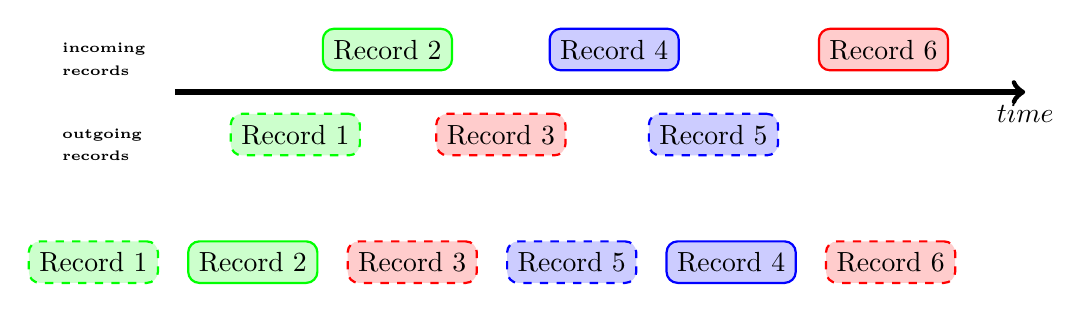
\begin{tikzpicture}[%
    scale=0.9,
    auto,
    block1/.style={
      rectangle,
      draw=blue,
      thick,
      fill=blue!20,
      text width=4em,
      align=center,
      rounded corners,
      minimum width=3em,
      minimum height=1.5em
    },
    block2/.style={
      rectangle,
      draw=green,
      thick,
      fill=green!20,
      text width=4em,
      align=center,
      rounded corners,
      minimum width=2em,
      minimum height=1.5em
    },
    block3/.style={
      rectangle,
      draw=red,
      thick,
      fill=red!20,
      text width=4em,
      align=center,
      rounded corners,
      minimum width=0.2em,
      minimum height=1.5em
    },
  ]
    \node[text width=3em] at (-2,-1.4) {\tiny\textbf{{incoming}}};
    \node[text width=3em] at (-2,-1.7) {\tiny\textbf{{records}}};
    \node[text width=3em] at (-2,-2.6) {\tiny\textbf{{outgoing}}};
    \node[text width=3em] at (-2,-2.9) {\tiny\textbf{{records}}};
    \draw [->,line width=0.7mm] (-1,-2) -- (11,-2) node[anchor=north] {$time$};
    \draw [dashed] (0.7,-2.6) node[block2] {Record 1};
    \draw (2,-1.4) node[block2] {Record 2};
    \draw [dashed] (3.6,-2.6) node[block3] {Record 3};
    \draw (5.2,-1.4) node[block1] {Record 4};
    \draw [dashed] (6.6,-2.6) node[block1] {Record 5};
    \draw (9,-1.4) node[block3] {Record 6};
    \draw [dashed] (-2.15,-4.4) node[block2] {Record 1};
    \draw (0.1,-4.4) node[block2] {Record 2};
    \draw [dashed] (2.35,-4.4) node[block3] {Record 3};
    \draw [dashed] (9.1,-4.4) node[block3] {Record 6};
    \draw [dashed] (4.6,-4.4) node[block1] {Record 5};
    \draw (6.85,-4.4) node[block1] {Record 4};
  \end{tikzpicture}
  \caption{An overview of \ac{TLS} record reordering (based on \cite{Mitseva2015})}
  \label{fig:tlsexample}
\end{figure}

In addition to \ac{TCP} data, we also extract \ac{TLS} records from the collected network traces. For that purpose, the script \texttt{raw-to-tls.py} extracts \ac{TLS} records from the original dump file using \texttt{tcpflow} and stores them in the form shown in Listing \ref{lst:tlsrawdata}. Then, similar to \texttt{parse-tcp.py}, the script \texttt{parse-tls.py} applies the \ac{IP} and timestamp matching to fetch the related connections only. In addition to the starting timestamp, \texttt{parse-tls.py} also extracts the timestamp of the \ac{TCP} packet containing the last \ac{TLS} segment as presented in Listing \ref{lst:tlsextracteddata}. This is necessary because a single \ac{TLS} record can be fragmented over multiple \ac{TCP} packets. Therefore, the data is reordered in a certain case: If a \ac{TLS} record, belonging to the communication with a given entry node, is being transferred in one direction and the transmission of a second record, belonging to the same communication, is started before the \ac{TCP} packet, containing the last fragment of the first record, is received, then the second \ac{TLS} record cannot be a response to the first record. % If a record is still being transmitted in one direction, a new record in the other direction cannot be a response to the ongoing, because it is not possible to process a record before all \ac{TCP} packets containing information regarding the same record have been received.
Figure~\ref{fig:tlsexample} illustrates an example of extracted \ac{TLS} records with their transmission time and direction. The colors of the records represent a communication with different entry nodes, i.e., in our example we consider three entry nodes. According to the duration of each transmission, we first start ordering records transferred from or to a certain entry node. Hence, we obtain the following pairs of records: 1,2 and 3,6 and 5,4. The data contained in record 4 cannot be a response of record 5 since the transmission of 4 has started before that of record 5. Afterwards, we start merging the reordered \ac{TLS} records. To do this, we compare the beginning of each \ac{TLS} record whereas we do not swap records belonging to the communication with the same entry node. In our example, we obtain the following sequence of records: 1,2,3,5,4,6. The script \texttt{parse-tls.py} does this reordering. If we enable to option \emph{legacy}, the script does not do reordering of the \ac{TLS} records, i.e., it considers the start timestamps only. 

\todo[inline]{Add newly added parsing scripts!}

\textcolor{red}{TODO: Describe the operation of check-hs-state.py, extract-main.py, parse-cells.py!}

At the end of our fetching process, the main script \texttt{fetch-and-calculate.sh} copies all collected and computed data into folder \texttt{fetches/} for further processing 

\todo[inline]{The data is copied in folder \texttt{storage/} not in \texttt{fetches/}!}

(see the organization of folder \texttt{fetches/} in Chapter \ref{chap:feature_generation}) and removes this data from folder \texttt{crawling/}. Thus, \texttt{crawling/} is ready for the next link list fetching.

\todo[inline]{Describe the option \emph{conf\_FUNCTION} located in \texttt{WFP\_config}!}

\textcolor{red}{TODO: Additionally, describe that we can either fetch traffic without processing the data or we can extract the different data layers without fetching page loads (in case that we have the collected traffic already and we want to recompute instances). Of course, the script can do both together.}

\todo[inline]{The following examples are all outdated!}
To illustrate the operation of our fetching algorithm, we consider a small example: First, we copy the generated \ac{URL} link list (see the example in Chapter 4) from folder \texttt{websiteCrawlingUrls/} into folder \texttt{crawling/}:
\vspace{-5mm}
\begin{verbatim}
# cp websiteCrawlingUrls/Urls.txt crawling/
\end{verbatim}
\vspace{-4mm}
\todo[inline]{And rename the file \texttt{Urls.txt} to \texttt{Urls}. Otherwise, you will have problems with the other scripts.}
Then, we start the main script for webpage fetching:
\vspace{-4mm}
\begin{verbatim}
# cd crawling/
# ./fetch-and-calculate.sh ../../WFP_config testRun 1 180 Urls.txt 
\end{verbatim}
\vspace{-4mm}
\todo[inline]{Show both possibilities with respect to the option \emph{conf\_FUNCTION} in \texttt{WFP\_config}!}
All measurements are directly saved into folder \texttt{fetches/} for further processing.

\section{Example files}
%\lstinputlisting[breaklines=true,language=Python,firstline=n1,lastline=n2, firstnumber=n3]{code/FILE}

\todo[inline]{Similar to the remark in Chapter~\ref{chap:list_generation}, check this example and reconstruct it in a way (if necessary) that we do not need to permanently store dummy files in the repository.}

\subsection{Input files}

The input file for fetching is the \texttt{Urls.txt} file that was created during link list creation. See Listing \ref{lst:inputUrls} for an example.

\subsection{Output files}

The following listing shows the output, consisting of the webpage \ac{URL}, timestamps and packet sizes, for the webpage \texttt{torproject.org}.
\begin{listing}[h!]
\caption{Input: \texttt{https\_\_\_www.torproject.org\_} (timestamps and sizes) \, (in folder \texttt{fetches/compiled/20150106\_121909\_test\_1\_180\_Urls\_mitseva-OptiPlex-960/output/})}
\lstinputlisting[breaklines=true,language=Python]{code/https___www.torproject.org_}
\label{lst:input1}
\end{listing}

\todo[inline]{Additional issues concerning fetching!}
\vspace{-5mm}
\begin{itemize}
  \item \textcolor{red}{Tor browser selenium (if you take a look in the old documentation, this is the previous Chickenfoot Script) which is used to manage a page load: In this script, there are different conditions used to check if a fetch is invalid (Source - the old documentation by Martin):}
  \begin{itemize}
    \item \textcolor{red}{$-1$ - Timeout (hard or soft) (needed, e.g., in case that the browser freezes)}
    \item \textcolor{red}{$-2$ - Empty page has been loaded (the \ac{URL} is about:blank)}
    \item \textcolor{red}{$-3$ - Firefox states that page has not loaded completely}
    \item \textcolor{red}{$-4$ - JavaScript Exception was thrown}
    \item \textcolor{red}{$-5$ - Waited too long for Tor streams to finish}
  \end{itemize}
\textcolor{red}{Over the years, the last condition \emph{Waited too long for Tor streams to finish} has disappeared. In the old documentation, there is no information how much one has to wait before considering a fetch as invalid. TODO: We need to revisit this!}
% check.torproject.org is removed! <-- \item \textcolor{red}{Do we still need the webpage \url{check.torproject.org}? When we load a page, we have two possibilities: $(i)$ We load foreground pages separately. This means after each foreground page (check.torproject.org + foreground page) the \ac{TBB} is restarted. $(ii)$ We load 10 background pages. This means that after 10 background pages (check.torproject.org + 10 background pages) the \ac{TBB} is restarted. In the past, the page \url{check.torproject.org} was necessary to check whether the Tor connection succeeded. Nevertheless, over the years \ac{TBB} has become much more stable. At the moment we are not using this page at all, but it is still loaded by the toolbox.}
% this is correct <-- \item \textcolor{red}{Do we correctly load a page? - After each page load, all Tor streams are closed. According to Tor specification, a circuit is closed if all streams on the corresponding circuit are closed and the lifetime of the circuit is over. Therefore, I am not sure if our foreground traces are really clean (i.e., they are loaded over a new circuit) since we first load the page \url{check.torproject.org}.}
  \item \textcolor{red}{The script \texttt{raw-to-tls.py} sometimes outputs memory error. The corresponding \ac{TLS} traces can not be extracted. Maybe problem in \texttt{tcpflow} or maybe not?}
  \item \textcolor{red}{The script \texttt{parse-tls.py} - Here, the extracting sometimes takes too long (2-3 days). Unfortunately, we did not manage to find and fix the problem.}
  \item \textcolor{red}{The scripts \texttt{check-fetches.py} and \texttt{clean-fetches.py} need improvement! They still do not clean all faulty traces.}
\end{itemize}


%!TEX root = ../documentation.tex
\chapter{Feature Generation}
\label{chap:feature_generation}

The feature generation is the essential part for our approach since we will not achieve good results with bad features during the classification. Our classifier can only work with the information it gets and the information that is available at that point in a real setting. Therefore, improving the features is more important than improving the classifier. In this chapter, we show how we generate features using the fetches already recorded. First, we introduce the organization of the folder \texttt{fetches/}. Then, we describe the operation of our feature generation algorithm and show a small example.

\section{Folder Organization}
\label{sec:feature_folder}

Our approach for generating features is located in the folder \texttt{fetches/}. Figure \ref{fig:fetchesOrdering} shows its organization. Folder \texttt{fetches/} consists of:

\begin{figure}
\dirtree{%
.1 \HandRight \, fetches.
.2 \HandRight \, features.
.3 \HandRight \, feature-<format>.
.4 \HandRight \, <webpage\_url>.
.3 $\star$ <dataSet>\_<format>.
.3 $\star$ list\_<dataSet>\_<format>.txt.
.2 \HandRight \, input.
.3 \HandRight \, <data>\_<runidentifier>\_<timeout>\_<urllist>.
.4 \HandRight \, <format>.
.5 \HandRight \, <webpage\_url>.
.2 \HandRight \, merged.
.3 \HandRight \, <format>.
.4 \HandRight \, <webpage\_url>.
.2 \HandRight \, outlierfree.
.3 \HandRight \, <format>-outlierfree.
.4 \HandRight \, <webpage\_url>.
.2 \HandRight \, scripts.
.3 $\star$ check-fetches.py.
.3 $\star$ clean-fetches-input.py.
.3 $\star$ generate-feature.py.
.3 $\star$ merge-input.sh.
.3 $\star$ outlier-removal.py.
.3 $\star$ Patterns.txt.
.2 \HandRight \, scriptsWang.
.3  $\star$  create-wang-cells-from-tls.py.
.3  $\star$  create-wang-cells-from-tls-legacy.py.
.2 \HandRight \, wang.
.3 \HandRight \, <format>-wang.
.4  $\star$  <webpage\_number>\_<instance\_number>.
.3  $\star$ Matching.txt.
.2 $\star$ TxtdumpErrors.txt.
}
\caption{Structure of folder \texttt{fetches/}}
\label{fig:fetchesOrdering}
\end{figure}

\todo[inline]{Add newly added formats and adjust fetches (incl. storage)!}
\begin{description}
\item[compiled/] A folder where the \ac{TCP} and \ac{TLS} instances generated during our webpage fetching process (see Chapter \ref{chap:webpage_fetching}) are saved. For that purpose, a new subdirectory with the name \texttt{<date>\_<runidentifier>\_<runs>\_<timeout>\_<urlfile>} is created for each fetching execution. Then, the folders \texttt{output/}, \texttt{output-tls/} and \texttt{output-tls-legacy/} with the corresponding files are copied from \texttt{crawling/} into this subdirectory.
\item [raw/] A folder where all subdirectories that contain collected and computed data from our webpage fetching algorithm are saved. Similar to \texttt{compiled/}, a new subdirectory with the name \texttt{<date>\_<runidentifier>\_<runs>\_<timeout>\_<urlfile>} is created for each fetching execution. Then, all folders with relevant information are copied from \textbf{crawling/} into this subdirectory (see Figure \ref{fig:fetchesOrdering}).
%\item[input/] This folder was manually created for merge-input.sh
\item[scripts/] A folder that contains all relevant scripts used for feature generation:
\begin{description}
\item[check-fetches.py] Verifies the webpage sources extracted during our webpage fetching algorithm (in the folder \texttt{txtdumps/}) for errors. For that reason, the \ac{HTML} code of each webpage is checked for predefined patterns that indicate a web failure. If any web failures are found, the corresponding \ac{TCP} and \ac{TLS} instances are removed.
\item[merge-input.sh] Merges \ac{TCP} and \ac{TLS} instances for a given webpage which are created by several fetching executions into a single file.
\item[outlier-removal.py] Removes outliers (see Section \ref{sec:feature_operation} for details).
\item[generate-feature.py] Generates features from the \ac{TCP} and \ac{TLS} instances previously prepared (see Section \ref{sec:feature_operation} for details).
\item[Patterns.txt] A text file that contains patterns for obvious transmission
errors. It is used by \texttt{check-fetches.py} to check the extracted webpage sources for web failures.
\item[TxtdumpErrors.txt] A text file that is generated only if the script \texttt{check-fet- ches.py} has removed any corrupted instances. It contains the name of the files where these instances were saved.
\end{description}
\item[features/] A folder used to store the generated features.
\item[merged/] A folder for the output of \texttt{merge-input.sh}, contains merged data from \texttt{compiled/}.
\begin{description}
\item[output/] A folder where the file(s) containing merged \ac{TCP} instances (merged by \texttt{merge-input.sh}) for a given webpage, which are created by several fetching executions, are saved.
\item[output-tls/] A folder where the file(s) containing merged \ac{TLS} instances with reordering (merged by \texttt{merge-input.sh}) for a given webpage, which are created by several fetching executions, are saved.
\item[output-tls-legacy/] A folder where the file(s) containing merged \ac{TLS} instances without reordering (merged by \texttt{merge-input.sh}) for a given webpage, which are created by several fetching executions, are saved.
\end{description}
\item[<reference\_dir>-outlierfree/] A directory containing the files that outlier removal shall be performed on.
\item[<process\_dir>-outlierfree/] If the user wants to remove all representation of faulty instances (see Section \ref{sec:feature_operation} for details), then a process directory has to be also defined. The process directory points to the folder(s) where the other formats of the corrupted instances are saved.
\end{description}

\section{Operation}
\label{sec:feature_operation}

Listing \ref{lst:generate_features} shows a summary of our feature generation approach. 

\begin{listing}[t]
Feature Generation Steps:
\begin{enumerate}
    \item Check extracted webpage sources for obvious transmission errors and remove corrupted \ac{TCP} and \ac{TLS} instances (\texttt{check-fetches.py}).
    %\item Copy all information from folder \texttt{compiled/} into folder \texttt{input/}. %No longer neccessary!
    \item Merge several \ac{TCP}, respectively \ac{TLS} instances for a given webpage into a single file (\texttt{merge-input.sh}).
    \item Remove outliers from merged files (\texttt{outlier-removal.py}).
    \item Generate features on outlier-free merged files (\texttt{generate-feature.py}).
\end{enumerate}
\caption{Summary of the feature generation approach}
\label{lst:generate_features}
\end{listing}

\subsection{Check fetches}
First, the webpage sources extracted during webpage fetching are verified for obvious transmission errors or page loads we do not want to use (\texttt{check-fetches.py}). For that purpose, we use predefined patterns (\texttt{Patterns.txt}) which indicate a possible web failure. \texttt{check-fetches.py} checks the content of a webpage source against our current patterns list. The script scans all instances located in the \texttt{storage/} directory.  The script generate an output file where the names of faulty instances are stored (\texttt{TxtdumpErrors.txt}). Afterwards the script \texttt{clean-fetches-input.py} removes the corresponding instances from all formats from the \texttt{input/} directory based on this list to not corrupt our classification result later. Therefore, the desired folders have to be copied from \texttt{compiled/} to \texttt{input/}. All parameters relevant to \texttt{check-fetches.py} and \texttt{clean-fetches-input.py} are located in the configuration file \texttt{WFP\_config} (see Appendix \ref{sec:config_file}), and can be adjusted before executing the script: 


\todo[inline]{Adjust the configuration options!}
\begin{description}
\item [fetches\_path] A folder that contains raw fetches. Typically, that is \texttt{\$HOME/WFA/ Implementation/fingerprinting/fetches/raw}.
\item [fetches\_pathcompiled] A folder that contains \ac{TCP} and \ac{TLS} instances created during webpage fetching. Typically, that is \texttt{\$HOME/WFA/Implementation/finger- printing/fetches/compiled}.
\item [closedWorld] Indicates if we consider closed-world (\texttt{true}) or open-world (\texttt{false}) scenario. \todo{Add what this option does}
\end{description}


\subsection{Merge instances}\label{Merge instances}
Afterwards, we merge all instances of the same format related to the same webpage, but collected during several fetching executions, into a single file (\texttt{merge-in- put.sh}). The script \texttt{merge-input.sh} creates folder \texttt{merged/} and folders for each format in \texttt{merged/} as output. Then, we check the merged instances for outliers and remove them based on the chosen metric (\texttt{outlier-removal.py}). 

\subsection{Remove outliers}\label{Remove outliers}
Outliers are instances, which feature extreme observation in comparison to instances of the same class. We regard the removal for each class in the closed-world and foreground class in the open-world scenario. This is reasonable due to the fact that Tor connections are error-prone. For example, the connection can time out before the transmission is finished because of a high load on the Tor circuit. A web server can be under a high load and can therefore skip the delivery of some files. In both cases the size of the recorded sample is smaller than it should be. A high network load can lead to many lost packets and therefore retransmissions, which lead to a higher transmission size. Such corrupt samples may tamper the trace in an undesired way. To avoid this, we search for outliers in the data and remove them. Our script \texttt{outlier-removal.py} provides three outlier detection algorithms.

\paragraph{Outlier detection algorithm proposed by Landa \cite{Landa2013}}
\label{par:landa_outlier}

The outlier detection proposed by Landa \cite{Landa2013} is three-stage process. First, all webpage instances with a incoming data size smaller or equal
two Tor cells are removed. This case can only happen, if there occurs an error during the transmission of the webpage. Second, a median of the incoming data sizes of all instances of a webpage is calculated. Then, we remove all instances where the incoming data size differs more than $0.8 \cdot median$ from the median. For example, this could be cases where the connection broke during the transmission or websites which had a huge advertisement in only very few instances. Third, we remove the outliers which are still in the data set. For that purpose, we calculate the first quartile $Q_{1}$ and the third quartile $Q_{3}$ of the incoming data sizes from the remaining instances for each webpage. Then, we remove all instances where the incoming data size does not fulfill the inequation shown in Listing \ref{lst:outlier}.

\paragraph{Outlier detection algorithm proposed by Pennekamp \cite{Pennekamp2014}}
\label{par:pennekamp_outlier}

The outlier detection proposed by Pennekamp \cite{Pennekamp2014} also excludes all webpage instances with a incoming data size smaller or equal
two Tor cells. Then, the algorithm computes the quantiles $Q_i$ regarding the incoming data of all instances belonging to a class and then removes all instances which do not satisfy the inequality in Listing \ref{lst:outlier}. Overall, we rely on "synchronized" instances while comparing results between different formats. This means that we want to use exactly the same traces in each format. For this reason, if the approach has to remove a faulty instance in one format (e.g., TCP), it removes that instance from all others as well (e.g., TLS). Pennekamp applies the outlier detection approach for each class in the closed-world and foreground class in the open-world scenario. For background instances, we do not care about unusual page loads because we are only interested in random web traffic. Incomplete or broken page loads are already removed by \texttt{check-fetches.py}.

\paragraph{Outlier detection algorithm proposed by Wang \cite{Wang2014}}
\label{par:wang_outlier}

\todo[inline]{Add Wang's outlier detection!}

\begin{listing}[t]
\caption{Outlier detection based on incoming data (based on \cite{Landa2013} and \cite{Pennekamp2014})}
\hrulefill\\[3mm]
\centering{
$Q_1 - 1.5 \cdot (Q_3 - Q_1) <  incomingData < Q_3 + 1.5 \cdot (Q_3 - Q_1)$}
\vspace{3mm}
\label{lst:outlier}
\end{listing}

All parameters relevant to \texttt{outlier-removal.py} are located in the configuration file \texttt{WFP\_config}, Section \texttt{[Outlier\_removal]} (see Appendix \ref{sec:config_file}), and can be adjusted before executing the script: 
\todo[inline]{Adjust the configuration variables, introduce command line parameter}
\begin{description}
\item [input\_outlier\_path] A path that points to files to which an outlier detection has to be applied. Typically, that is \texttt{\$HOME/WFA/Implementation/fingerprinting/ fetches/}.
\item [ignore\_outlier] If set to \texttt{false} all outliers will be removed, even if this means that \texttt{num\_of\_wished\_instances} is undershot. Contrary, if set to \texttt{true} only as many outliers as possible will be removed without undershooting \texttt{num\_of\_wished\_instances}. Setting \texttt{ignore\_outlier} to \texttt{true} thus ensures that the number of instances is never lower than \texttt{num\_of\_wished\_instances} at the cost that some outliers will remain in the data set.
\item [outlier\_removal] Indicates the type of the selected outlier detection algorithm. We can select \texttt{Simple} - outlier detection proposed by Pennekamp (see \ref{par:pennekamp_outlier}), \texttt{Strict} - outlier detection proposed by Landa (see \ref{par:landa_outlier}) or \texttt{Wang} - outlier detection proposed by Wang (see \ref{par:wang_outlier}).
\item [num\_of\_wished\_instances] The number of wished instances that the script has to output. Note, that this number has to be equal or larger than the number of instances in all input files. \textbf{If one input file has less instances, the script will abort with an error.}
\item[random\_instances] Indicates whether consider the instances randomly or e.g., we consider the first 60, 80, etc.
\item [reference\_dir] A directory containing the files that outlier removal shall be performed on. The path to this directory is relative starting from \texttt{input\_outlier\_path}.
\end{description}
If the user wants to remove all representation of faulty instances, e.g., if a certain \ac{TCP} instance is corrupted and the user wants to remove its corresponding \ac{TLS} instance as well, then a \emph{process directory} has to be also defined. For that purpose, the following code line in \texttt{outlier-removal.py} has to be enabled:
\begin{verbatim}
# By default, we delete only these instances 
# that the outlier-removal was performed on
# Disable this line if you want to remove 
# all representation of faulty instances
# processDirectories = []

# All directories that should have the same instances 
# removed, separated via commata.
processDirectories = [ 'output-tls', 'output-tls-legacy' ]
\end{verbatim}
As a result, the same instances that are removed for files in the reference directory are also removed from the files in the process directory(s). The output files from \texttt{outlier-removal.py} are saved in the automatically generated folder(s) \texttt{<reference\_dir>-outlierfree/} and \texttt{<process\_dir>-outlierfree/} if \texttt{process\_dir} is previously defined (see Figure \ref{fig:fetchesOrdering}).

\subsection{Generate features}

After we have deleted the instances that may corrupt or influence our classification later, we start generating features using \texttt{generate-feature.py}.
\begin{verbatim}
usage: python generate-feature.py
\end{verbatim}
This script provides two feature generation approaches:

\paragraph{Cumulative Version}
\label{par:cumulative_version}

In our cumulative version, we rely on a feature which consists of 100 values to store the trace as accurate as possible. These 100 values are computed from the chronological sequence of incoming and outgoing packets. In order to compose the features, we use the \ac{TCP}, respectively \ac{TLS}, data tuples previously prepared. Thus, we compute a plot and take \emph{n} values with the same distance to each other from the plot. In order to calculate the plot, first we have to calculate two arrays: the absolute size and the cumulated size. The absolute size is the sum of all absolute packet sizes added up:
\begin{center}
\hspace{-60mm}$absoluteSize[0] = abs(data[0])$\\
\hspace{-10mm}$absoluteSize[i] = absoluteSize[i - 1] + abs(data[i])$, $i \geq 1$
\end{center}
We calculate the cumulated size array in a similar way, but we subtract the outgoing traffic instead of adding it:
\begin{center}
\hspace{-90mm}$cumulatedSize[0] = data[0]$\\
$cumulatedSize[i] = data[i].isOutgoingData$ ? $cumulatedSize[i - 1] - abs(data[i]) :$\\
\hspace{-50mm}$cumulatedSize[i - 1] + abs(data[i]), i \geq 1$
\end{center}
After the calculation of the arrays, we interpolate a plot from the value pairs (\emph{absoluteSize[i]},\emph{cumulatedSize[i]}) and calculate 100 sample values with the same distance to each other. 
\todo[inline]{May be, pictures have to be added as well?!}

\paragraph{Separate Version}
\label{par:separate_version}

In comparison to the cumulative version, in the separate version we divide the information regarding the stream of incoming and outgoing packets. In detail, instead of subtracting outgoing packet sizes for the incoming cumulative list, we duplicate the previous entry. Accordingly, the outgoing cumulative list does not accumulate incoming packet sizes. In order to not lose information in comparison to the cumulative version, we have to increase the overall number of sampling points. Given that we have twice the cumulative length, we simply double the amount from 100 to 200 and interpolate each list like before to obtain our desired 200 sampling points. 
\todo[inline]{May be, pictures have to be added as well?!}

Finally, \texttt{generate-feature.py} transforms the generated features into a format the \ac{SVM} can work with (see Chapter \ref{chap:classification} for details).

\todo[inline]{Adjust the configuration variables, introduce command line parameter}
Before executing \texttt{generate-feature.py}, several parameters within \texttt{WFP\_config} (see Appendix \ref{sec:config_file}), have to be adjusted:
\begin{description}
\item[input\_path] A path that points to directories to which an the feature generation algorithm has to be applied. Typically, that is \texttt{\$HOME/WFA/Implementation/finger- printing/fetches/}.
\item[fetch\_input] A directory containing the files that the feature generation algorithm shall be performed on. The path to this directory is relative starting from \texttt{input\_path}.
\item[feature\_output] A folder where the files with the generated features are saved. Typically, this folder is a subdirectory of folder \texttt{features/} (see Figure \ref{fig:fetchesOrdering}).
\item[feature\_name] A name of a file containing a generated feature.
\item[num\_of\_wished\_instances] The number of instances that the script will output. Note that this number has to be equal or larger than the number of instances in all input files. \textbf{If one input file has less instances, the script will abort with an error.} Typically, this number is the same as \texttt{num\_of\_wished\_instances} in section \texttt{[Outlier-removal]}, but it might be also lower. An example for the latter would be that outlier removal is performed for 100 instances, but features should be generated for 60, 80 and 100 instances.

\textbf{Note, that if the number of valid instances is less than \texttt{num\_of\_wished\_instances}, then no (complete) output is generated. On the terminal, the user will get the following error message:}
\begin{verbatim}
WARN: output-tls/https___cloud.torproject.org_ only 5/5 of 6
ERROR: output-tls/https___cloud.torproject.org_ only 5/5 of 6
\end{verbatim}
\item[feature\_count] A number of features, e.g., 100, 200. Note, that it should be even. % add check into script for that
\item[setting] Indicates if we consider open-world foreground (\texttt{OW\_FG}), open-world background (\texttt{OW\_BG}) or closed-world (\texttt{CW}). \todo[inline]{Explain the difference between the scenarios!}
\item[separate\_classifier] Shows if we generate separate version (\texttt{true}) or cumulative version (\texttt{false}).
\item[random\_instances] This variable may be either \texttt{true} or \texttt{false}. If it is set to \texttt{true}, the instances used for feature generation are taken at random. Otherwise, they are taken sequentially starting at instance 1.
\item[data\_set] Can be freely chosen or is set to \texttt{\#}. If a name other than \texttt{\_} is chosen, a single file will be created as output. If \texttt{\_} is chosen, for each webpage a file will be created.
\end{description}

\todo[inline]{The following examples are all outdated!}
To illustrate the operation of our feature generation approach, we consider a small example. After we have finished the execution of \texttt{fetch-and-calculate.sh} (see Chapter \ref{chap:webpage_fetching} for details), we move into folder \texttt{fetches/} and remove all transmission errors from the instances previously generated:
\begin{verbatim}
# cd ../fetches
# cd scripts/
# ./check-fetches.py
\end{verbatim}

Afterwards, we merge all \ac{TCP}, respectively \ac{TLS}, instances for a given webpage into a single file:
\begin{verbatim}
# ./merge-input.sh
\end{verbatim}
The output files of \texttt{merge-input.sh} are located in the subfolders \texttt{output/}, \texttt{output-tls/}, \texttt{output-tls-legacy/}, \texttt{output-cells/}, \texttt{output-cells-sendme/} and \texttt{output-tls-no- sendme/} of folder \texttt{merged/}, as we have already described (see Section \ref{Merge instances}).

Then, we execute \texttt{outlier-removal.py} to remove all outliers:
\begin{verbatim}
# ./outlier-removal.py
\end{verbatim}
The output from this script is saved in folder(s) \texttt{<reference\_dir>-outlierfree/} and \texttt{<process\_dir>-outlierfree/} if \texttt{process\_dir} is previously defined (see Section \ref{Remove outliers}).

Finally, we generate our features:
\begin{verbatim}
# ./generate-feature.py
\end{verbatim}
The output files from this example can be found in the folder \texttt{fetches/}. Appendix \ref{sec:config_file} shows the configuration file that we use.

The output of \texttt{generate-feature.py} is structured as follows: Each instance is stored in a single line starting with a number indicating the current class label and followed by the corresponding features. In the closed-world scenario, each class has a different unique label. Additionally, every class has the same number of instances and all classes are stored in one file. The classification performed for the closed-world scenario is called an \emph{all-vs-all} approach since each class is evaluated against any other. On the other hand, our open-world scenario follows an \emph{one-vs-all} approach also known as \emph{one-vs-rest} approach. For that purpose, we have separate files for each foreground class. Instances belonging to the foreground are labeled as class \texttt{1} while any instance in the background is labeled as class \texttt{0}. In the background we do not differentiate between different domains because we simply want to determine whether the current instance is an interesting one, i.e., belonging to the foreground, or not. Overall, we obtain two classes in each input file for the open-world scenario. 

The features for both scenarios are stored in the following format $i$:\emph{Feature}$_i$ where $i$ denotes the number of the current feature and \emph{Feature}$_i$ represents the value of the $i$-th feature. See Listing \ref{lst:outputTorprojectFeatures} for an example.


%\pagebreak
\section{Example files}
%\lstinputlisting[breaklines=true,language=Python,firstline=n1,lastline=n2, firstnumber=n3]{code/FILE}

\subsection{Input files}
Listing \ref{lst:input1} shows an exemplary input file for \texttt{generate-feature.py}. Its content consists of the URL that was fetched, and timestamps and packet sizes that occurred during fetching.

\subsection{Output files}
\todo[inline]{Add appended timestamp as comment in generated feature files}
After running \texttt{generate-feature.py} on the input files, the resulting feature file for \texttt{torproject.org} looks like shown in Listing \ref{lst:outputTorprojectFeatures}.
\begin{listing}[h!]
\caption{Output: \texttt{https\_\_\_www.torproject.org\_} (features) (in folder \texttt{fetches/features/output/})}
\lstinputlisting[breaklines=true,language=Python]{code/https___www.torproject.org_FEATURES}
\label{lst:outputTorprojectFeatures}
\end{listing}

\subsection{Input files - closed world}\label{sec:Input files - closed-world}
For closed-world classification files like shown in Listing \ref{lst:input1} with (typically) more than one line are used. See Listing \ref{lst:input2} for a more realistic example.

\begin{listing}[h!]
\caption{Input: \texttt{http\_\_\_www.facebook.com\_} (timestamps and sizes)}
\lstinputlisting[breaklines=true,language=Python]{code/http___www.facebook.com_}
\label{lst:input2}
\end{listing}

\subsection{Output files - closed-world}
In closed-world classification each webpage is assigned an own class. In Listing \ref{lst:output1} the features for \texttt{facebook.com} are shown. The class value is 17, since \texttt{facebook.com} happened to be the 17th webpage used to generate features for. Note that here the number of instances for which features were generated is lower than the number of instances in the input file (as shown in Listing \ref{lst:input2}). Additionally note that this example is taken from a real classification run, so originally there are 104 features for each instance.

\begin{listing}[h!]
\caption{Output (CW): \texttt{http\_\_\_www.facebook.com\_} (features)}
\lstinputlisting[breaklines=true,language=Python]{code/http___www.facebook.com_FEATURES}
\label{lst:output1}
\end{listing}

\subsection{Input files - open-world}
The input files for open-world classification are the same as for closed-world classification. Thus, see Section \ref{sec:Input files - closed-world} for an example.

\subsection{Output files - open-world}
Contrary to closed-world we do not enumerate the webpages in open-world classification. Instead, we differentiate between \ac{FG} and \ac{BG} webpages. Webpages belonging to \ac{FG} get class label 1, those belonging to \ac{BG} get class label 0.

Let us consider three webpages, from which one is monitored (thus it belongs to \ac{FG}) and two are non-monitored (belonging to \ac{BG}). In closed-world classification the resulting features look like in Listing \ref{lst:output2}. For open-world classification the results are shown in Listing \ref{lst:output3} (\ac{FG}) and Listing \ref{lst:output4} (\ac{BG}).

\begin{listing}[h!]
\caption{Output (CW): artificial example (features)}
\lstinputlisting[breaklines=true,language=Python]{code/features_CW.txt}
\label{lst:output2}
\end{listing}

\begin{listing}[h!]
\caption{Output (OW\_FG): artificial example (features)}
\lstinputlisting[breaklines=true,language=Python]{code/features_OW_FG.txt}
\label{lst:output3}
\end{listing}

\begin{listing}[ht!]
\caption{Output (OW\_BG): artificial example (features)}
\lstinputlisting[breaklines=true,language=Python]{code/features_OW_BG.txt}
\label{lst:output4}
\end{listing}

For training of a classifier we need a single input file, so the two files for open-world \ac{FG} and \ac{BG} need to be merged. Thus, the result of feature generation for open-world scenarios needs to look like in Listing \ref{lst:output5}. Note that the differentiation between \ac{FG} and \ac{BG} needs to be done manually.

\begin{listing}[ht!]
\caption{Output (OW): artificial example (features)}
\lstinputlisting[breaklines=true,language=Python]{code/features_OW.txt}
\label{lst:output5}
\end{listing}
%!TEX root = ../documentation.tex
\chapter{Classification}
\label{chap:classification}

After we generated the features for each webpage, we need to train a classifier on it. For that purpose we use LIBSVM\footnote{\url{http://www.csie.ntu.edu.tw/~cjlin/libsvm/}}, a library for SVMs. LIBSVM provides us with two possibilities to train and test a classifier: manual and automated. If done manually, the user needs to
\begin{itemize}
\item Scale the data,
\item Choose a kernel,
\item Determine the kernel's best parameters,
\item Train the SVM using those parameters and the training data,
\item Test the SVM on the training data.
\end{itemize}

More information can be found in the guideline\footnote{\url{http://www.csie.ntu.edu.tw/~cjlin/papers/guide/guide.pdf}} for beginners, published by Hsu et al.

LIBSVM is located in folder \texttt{evaluation/}. See Figure \ref{fig:evaluationFolder} for its structure.

\begin{figure}
\dirtree{%
.1 \HandRight \, evaluation.
.2 \HandRight \, <folder>.
.2 $\star$ <file>.
}
\caption{Structure of folder \texttt{evaluation/} \todo[inline]{Adjust structure to represent the real implementation!}}
\label{fig:evaluationFolder}
\end{figure}

For an easier start with classification, the process outlined above is completely automated by the script \texttt{easy.py} (can be found in folder \texttt{tools/} in \texttt{libsvm-3.20}). This script only needs a training file and optionally takes a testing file. 
\begin{verbatim}
usage: ./easy.py training_file [testing_file]

     Program for automated classification.

training file        Dataset used for training the SVM.
[testing file]       Dataset used for testing the SVM (optional).
                     Instances in testing file have to be
                     distinct from instances in training file!
\end{verbatim}

Given training and testing files, \texttt{easy.py} trains an SVM according to the process given above and tests it using the data in the testing file. If no testing file is provided, \texttt{easy.py} uses cross-validation. The training file needs to consist of all instances that shall be used for training. Similar, for testing the testing file needs to consist of all those instances intended for testing. As \texttt{generate-feature.py} might have created one output file per webpage, depending on the settings, one needs to merge the output into one file. The resulting file should look like Listing \ref{lst:output2} for \ac{CW} and Listing \ref{lst:output5} for \ac{OW}, respectively.

For this documentation we will limit ourselves to automated classification with \texttt{easy.py}. Note that we have created several enhancements of \texttt{easy.py}, each of which is intended to be used for a special use-case only. \todo[inline]{Which scripts shall be included in the folder, which of them should maybe be explained here or in the appendix?}

\section{Small example for usage of \texttt{easy.py}}

In the following we will show a small example using the data from Listing \ref{lst:output2} which we save in a file \texttt{features\_CW}. This file is copied into the \texttt{tools/}-folder where \texttt{easy.py} is located. Then we execute \texttt{easy.py} with \texttt{features\_CW} as input file.

\begin{verbatim}
./easy.py features_CW 
Scaling training data...
Cross validation...
Best c=0.03125, g=0.0078125 CV rate=33.3333
Training...
Output model: features_CW.model
\end{verbatim}

As we do not input a file for testing, \texttt{easy.py} performes cross-validation on the training data. The output shown above gives us the resulting parameters for the SVM and the accuracy (rate) in the third line of output:
\begin{verbatim}
Best c=0.03125, g=0.0078125 CV rate=33.3333
\end{verbatim}

Furthermore, \texttt{easy.py} outputs the classifier model \texttt{features\_CW.model}. This is the \emph{classifier} which can be used in \texttt{svm-predict} to classify new test data.

\todo[inline]{Enhance file management of Eval scripts!}

\textbf{OLD STUFF:}\\
%After generating the features for each webpage trace, we have to input the data into the classifier. For classification we use LIBSVM, the data has to be in a certain format. Therefore, we have performed a certain preprocessing of the features using \texttt{generate-feature.py}. We have stored our generated instances and the matching features accordingly. Each instance is stored in a single line starting with a number indicating the current class label and followed by the corresponding features. In the closed-world scenario, each class has a different unique label. Additionally, every class has the same number of instances and all classes are stored in one file. The classification performed for the closed-world scenario is called an \emph{all-vs-all} approach since each class is evaluated against any other. On the other hand, our open-world scenario follows an \emph{one-vs-all} approach also known as \emph{one-vs-rest} approach. For that purpose, we have separate files for each foreground class. Instances belonging to the foreground are labeled as \texttt{Class 1} while any instance in the background is labeled as \texttt{Class 0}. In the background we do not differentiate between different domains because we simply want to determine whether the current instance is an interesting one, i.e., belonging to the foreground, or not. Overall, we obtain two classes in each input file for the open-world scenario. The features for both scenarios are stored in the following format $i:Feature_i$ where $i$ denotes the number of the current feature and $Feature_i$ represents the value of the $i$-th feature.

%\todo{To filter and remove pages with the same domain from our background data sets in the open-world scenario, we use the Python package tldextract. --> This is done by \texttt{Process.py} that we do not use. May be we stll need some parts from this script?}
\todo[inline]{Add Process.py to explain Open World Eval}
%!TEX root = ../documentation.tex
\chapter{Wang's Fingerprinting Approach}
\label{chap:wang}

\todo[inline]{Include a section to present the WFP attack proposed by Wang and our scripts to compare the results?!}

%!TEX root = ../documentation.tex
\chapter{Demo}
\label{chap:example}

\todo[inline]{The following chapter is completely outdated!}
In this Chapter, we introduce a small demo of our \ac{WF} attack that demonstrates the main execution steps.

First, we negotiate the parameters in the file \texttt{parameters.cfg} (see Appendix \ref{sec:config_file}) and load our configuration file \texttt{WFP\_config}.
\begin{verbatim}
# ./WFP_config
\end{verbatim}
Next, we start generating a valid \ac{URL} link list:
\begin{verbatim}
# cd websiteCrawlingUrls/
\end{verbatim}
We enter the following list of websites in the input file \texttt{URL\_Lists.txt}:\\[1mm]
\url{http://rwth-aachen.de}\\
\url{http://google.de}\\
\url{http://www.torproject.org/}\\
\url{http://heise.de}\\
\url{http://golem.de}

Afterwards, we start the script:
\begin{verbatim}
# python CrawlSite.py
\end{verbatim}
The script retrieves several subpages for each \ac{URL} and stores them in the corresponding output files:\\[1mm]
fetches\_rwth-aachen.de.txt\\
fetches\_google.de.txt\\
fetches\_torproject.org.txt\\
fetches\_heise.de.txt\\
fetches\_golem.de.txt

Finally, we merge these output files into one called \texttt{Urls.txt}:
\begin{verbatim}
# cat fetches_* > Urls.txt
\end{verbatim}

We copy the generated \ac{URL} link list into folder \texttt{crawling/} and move into \texttt{crawling/} to perform webpage fetching:
\begin{verbatim}
# cp Urls.txt ../crawling/
# cd ../crawling/
\end{verbatim}
Then, we start the main script for webpage fetching:
\begin{verbatim}
# ./fetch-and-calculate.sh ../../WFP_config testRun 1 180 Urls.txt 
\end{verbatim}
All measurements are directly saved into folder \texttt{fetches/}. We move into folder \texttt{fetches/} and check the generated fetches for web failures:
\begin{verbatim}
# cd ../fetches/
# cd scripts/
# ./check-fetches.sh
\end{verbatim}

Afterwards, we merge all \ac{TCP}, respectively \ac{TLS}, instances for a given webpage into a single file:
\begin{verbatim}
# ./merge-input.sh
\end{verbatim}
The output files of \texttt{merge-input.sh} are located in the subfolders \texttt{output/}, \texttt{output-tls/}, \texttt{output-tls-legacy/}, \texttt{output-cells/}, \texttt{output-cells-sendme/} and \texttt{output-tls-no- sendme/} of folder \texttt{merged/}, as we have already described (see Section \ref{Merge instances}).

Then, we execute \texttt{outlier-removal.py} to remove all outliers: 
\begin{verbatim}
# ./outlier-removal.py
\end{verbatim}
The output from this script is saved in folder(s) \texttt{<reference\_dir>-outlierfree/} and \texttt{<process\_dir>-outlierfree/} if \texttt{process\_dir} is previously defined (see Figure \ref{fig:fetchesOrdering}).

Finally, we generate our features:
\begin{verbatim}
# ./generate-feature.py
\end{verbatim}
According to our configuration file (see Appendix \ref{sec:config_file}), our generated features are saved in folder \texttt{features/}.

Having the features generated, we need to make sure that the instances are in the correct input files for classification. This usually means that the files containing the feature values need to be merged into one file that we use as training data. 

\begin{verbatim}
# cd ../features/output
# cat * > merged_feature_files
\end{verbatim}

The file \texttt{merged\_feature\_files} can now be used for classification. For that we copy the file to the folder \texttt{evaluation/input/}. Then we change to the \texttt{tools/}-folder in which \texttt{easy.py} is located and let it run on \texttt{merged\_feature\_files}. Since the output files are create within \texttt{tools/} we finally move them up to the folder \texttt{evaluation/output/}.

\begin{verbatim}
# cp merged_feature_files ../../../evaluation/input/
# cd ../../../evaluation/libsvm-3.20/tools/
# ./easy.py ../../input/merged_feature_files 
Scaling training data...
Cross validation...
Best c=0.03125, g=0.0078125 CV rate=0.0
Training...
Output model: merged_feature_files.model
# mv merged_feature_files.* ../../output/
\end{verbatim}

%  \item Check the generated fetches for corrupt instances through:
%\begin{verbatim}
%cd fetches/scripts/
%python check-fetches.py
%\end{verbatim}
%  \item To generate features we first need to set the input path in \textbf{parameters.cfg}, section [Features], to the newly created folder in \textbf{fetches/compiled}: 
%  \begin{verbatim}
%  input_path: /home/mitseva/Documents/Implementation/fingerprinting/
%              fetches/compiled/20141020_173459_1_10_200_Urls/
%  \end{verbatim}
  
%  Then generate features through:
%\begin{verbatim}
%python generate-feature.py
%\end{verbatim}
%The output of feature generation can be seen in a folder \textbf{fetches/features}. Using this output, we represent the generated features for the webpage \emph{http://rwth-aachen.de} graphically as shown in Figure \ref{fig:rwthaachen_tcp}.
%\end{enumerate}

%\begin{figure}
% \centering
%  \subfigure[Separate version]{
%  \centering
%   \begin{tikzpicture}[scale=1]
%     \begin{axis}[
%       height=7cm,
%       width=8cm,
%       xlabel={feature number},
%       ylabel={feature value},
%       legend pos=outer north east,
%       enlarge x limits=false,
%       scaled x ticks = false,
%       xtick={1,25,50,75,100},
%       xticklabel style={/pgf/number format/fixed},
%       scaled y ticks = false,
%       yticklabel style={/pgf/number format/fixed}]
%       \addplot[color=red, mark=none] table [x=feature, y=1, col sep=comma]%{pictures/rwthAachen_sep_tcp.csv};
%       \addplot[color=green, mark=none] table [x=feature, y=2, col sep=comma] {pictures/rwthAachen_sep_tcp.csv};
%       \addplot[color=blue, mark=none] table [x=feature, y=3, col sep=comma] {pictures/rwthAachen_sep_tcp.csv};
%       \addplot[color=cyan, mark=none] table [x=feature, y=4, col sep=comma] {pictures/rwthAachen_sep_tcp.csv};
%       \addplot[color=magenta, mark=none] table [x=feature, y=5, col sep=comma] {pictures/rwthAachen_sep_tcp.csv};
%       \addplot[color=orange, mark=none] table [x=feature, y=6, col sep=comma] {pictures/rwthAachen_sep_tcp.csv};
%       \addplot[color=black, mark=none] table [x=feature, y=7, col sep=comma] {pictures/rwthAachen_sep_tcp.csv};
%       \addplot[color=brown, mark=none] table [x=feature, y=8, col sep=comma] {pictures/rwthAachen_sep_tcp.csv};
%       \addplot[color=lime, mark=none] table [x=feature, y=9, col sep=comma] {pictures/rwthAachen_sep_tcp.csv}; 
%\end{axis}
%\end{tikzpicture}
%}
%\subfigure[Cumulative version]{
%  \centering
%   \begin{tikzpicture}[scale=1]
%     \begin{axis}[
%       height=7cm,
%       width=8cm,
%       xlabel={feature number},
%       ylabel={feature value},
%       legend pos=outer north east,
%       enlarge x limits=false,
%       scaled x ticks = false,
%       xtick={1,25,50,75,100},
%       xticklabel style={/pgf/number format/fixed},
%       scaled y ticks = false,
%       yticklabel style={/pgf/number format/fixed}]
%       \addplot[color=red, mark=none] table [x=feature, y=1, col sep=comma]%{pictures/rwthAachen_cum_tcp.csv};
%       \addplot[color=green, mark=none] table [x=feature, y=2, col
%sep=comma] {pictures/rwthAachen_cum_tcp.csv};
%       \addplot[color=blue, mark=none] table [x=feature, y=3, col sep=comma] {pictures/rwthAachen_cum_tcp.csv};
%       \addplot[color=cyan, mark=none] table [x=feature, y=4, col sep=comma] {pictures/rwthAachen_cum_tcp.csv};
%       \addplot[color=magenta, mark=none] table [x=feature, y=5, col sep=comma] {pictures/rwthAachen_cum_tcp.csv};
%       \addplot[color=orange, mark=none] table [x=feature, y=6, col sep=comma] {pictures/rwthAachen_cum_tcp.csv};
%       \addplot[color=black, mark=none] table [x=feature, y=7, col sep=comma] {pictures/rwthAachen_cum_tcp.csv};
%       \addplot[color=brown, mark=none] table [x=feature, y=8, col sep=comma] {pictures/rwthAachen_cum_tcp.csv};
%       \addplot[color=lime, mark=none] table [x=feature, y=9, col sep=comma] {pictures/rwthAachen_cum_tcp.csv}; 
%\end{axis}
%\end{tikzpicture}
%}
%\caption{http://rwth-aachen.de}
%\label{fig:rwthaachen_tcp}
%\end{figure}



%%%%%%%%%%%%%%%%%%%%%%%%%%%%%%%%%%%%%%%%%%%%%%%%%%%%%%%%%%%%%
%% LITERATUR
%%%%%%%%%%%%%%%%%%%%%%%%%%%%%%%%%%%%%%%%%%%%%%%%%%%%%%%%%%%%%

\phantomsection
\addcontentsline{toc}{chapter}{Bibliography}
%\nocite{*}								
\bibliography{literature/literature}
\bibliographystyle{styles/acmurl}


%%%%%%%%%%%%%%%%%%%%%%%%%%%%%%%%%%%%%%%%%%%%%%%%%%%%%%%%%%%%%
%% ANHÄNGE
%%%%%%%%%%%%%%%%%%%%%%%%%%%%%%%%%%%%%%%%%%%%%%%%%%%%%%%%%%%%%
\appendix
%!TEX root = ../documentation.tex
\chapter{Appendix}
\section{Abbreviations}
\label{sec:abbreviations}

\begin{acronym}[ABCDEFGH]
	\setlength{\itemsep}{-\parsep}
	\acro{API}{Application Programming Interface}
	\acro{BG}{background}
	\acro{CV}{Cross-validation}
	\acro{CW}{closed-world}
	\acro{FG}{foreground}	
	\acro{FN}{False Negatives}
	\acro{FP}{False Positives}
	\acro{HTML}{HyperText Markup Language}
	\acro{HTTP}{Hypertext Transfer Protocol}
        \acro{HS}{Hidden Service}
	\acro{IP}{Internet Protocol}
	\acro{OS}{Operating System}
	\acro{OW}{open-world}
	\acro{SSL}{Secure Sockets Layer}
	\acro{SVM}{Support Vector Machine}
	\acro{TA}{Traffic Analysis}
	\acro{TBB}{Tor Browser Bundle}
	\acro{TCP}{Transmission Control Protocol}
	\acro{TLS}{Transport Layer Security}
	\acro{TN}{True Negatives}
	\acro{Tor}{Anonymization network, previously abbreviation for The Onion Router}
	\acro{TP}{True Positives}
	\acro{URL}{Uniform Resource Locator}
	\acro{WFP}{Website Fingerprinting}
        \acro{WWW}{World Wide Web}
\end{acronym}

%!TEX root = ../documentation.tex
\section{Configuration File}
\label{sec:config_file}

\begin{verbatim}
#!/bin/bash

# setting variables globally
set -a

#######################################################################
#######################################################################
#
# The following lines have to be adjusted according to the
# user's configuration.
#
#######################################################################
#######################################################################

##########################################
# Username
##########################################
conf_USER="mitseva"

##########################################
# An interface which tcpdump listens on
##########################################
conf_ETHDEVICE="eth0"

##########################################
# Home directory
##########################################
dir_HOME=$HOME

##########################################
# Main directory containing all tools
##########################################
dir_MAIN="${dir_HOME}/Documents/wfp_toolbox/WFP_Implementation/fingerprinting/"



#######################################################################
#######################################################################
# URL list generation
#######################################################################
#######################################################################

##########################################
# Firefox Profile
##########################################
dir_FF_PROFILE="/home/fop/.mozilla/firefox/ddmr1z3e.default"

##########################################
# Number (!) of Subpages to be Generated
##########################################
conf_SUBPAGES="5"

##########################################
# Timeout (in Seconds) for each Page Load
##########################################
conf_PAGELOAD_TIMEOUT="20"

##########################################
# Input Linklist for Subpage Generation
##########################################
file_URLList="./URL_List.txt"



#######################################################################
#######################################################################
# Fetch Processing (including Outlier Removal) & Feature generation
#######################################################################
#######################################################################

##########################################
# Patterns to be checked in traces
##########################################
conf_PATTERNS="Patterns.txt"

##########################################
# Clean transmission errors from traces representing background
##########################################
# available options: YES | NO
conf_DEL_TRANSMISSION_ERR="YES"
#conf_DEL_TRANSMISSION_ERR="NO"

##########################################
# Reference Format for synchronized Outlier Removal
##########################################

# available options: tcp | tls | tls-legacy | tls-nosendme | 
# 						cell | cell-nosendme | 
#						cell-legacy | cell-nosendme-legacy
#conf_OUTLIER_REFERENCE="tcp"
conf_OUTLIER_REFERENCE="tcp"
#conf_OUTLIER_REFERENCE="tls"
#conf_OUTLIER_REFERENCE="tls-legacy"
#conf_OUTLIER_REFERENCE="tls-nosendme"
#conf_OUTLIER_REFERENCE="cell"
#conf_OUTLIER_REFERENCE="cell-nosendme"
#conf_OUTLIER_REFERENCE="cell-legacy"
#conf_OUTLIER_REFERENCE="cell-nosendme-legacy"

##########################################
# "Strictness" of Outlier Removal
##########################################
# available options: Simple | Strict | Wang
conf_OUTLIER_REMOVAL="Simple"
#conf_OUTLIER_REMOVAL="Strict"
#conf_OUTLIER_REMOVAL="Wang"

##########################################
# Ignore Outlier Removal if necessary
##########################################
# available options: YES | NO
#conf_IGNORE_OUTLIER="YES"
conf_IGNORE_OUTLIER="NO"

##########################################
# Evaluated Scenario (Class Labeling differs)
##########################################
# available options: CW | OW_FG | OW_BG
conf_SETTING="CW"
#conf_SETTING="OW_FG"
#conf_SETTING="OW_BG"

##########################################
# Number (!) of Instances per Webpage
##########################################
conf_INSTANCES="40"

##########################################
# Take Random Instances if Possible
##########################################
# available options: YES | NO
conf_RANDOM_INSTANCES="YES"
#conf_RANDOM_INSTANCES="NO"

##########################################
# Used Classifier Version to Generate Features
##########################################
# available options: CUMULATIVE | SEPARATE
conf_CLASSIFIER="CUMULATIVE"
#conf_CLASSIFIER="SEPARATE"

##########################################
# Number (!) of Features per Instance (has to be even)
##########################################
conf_FEATURES="100"

##########################################
# Features are Outputted in a Single File or in Directories
##########################################
# available options: _ [Directories] | *Name* [Single File]
conf_DATASET="_"



#######################################################################
#######################################################################
# Choose functionality
#######################################################################
#######################################################################
# available options: ALL | FETCH | CALCULATE | FETCH_AND_CALCULATE | 
#					 CHECK_HS_STATE | CALCULATE_FEATURES
#conf_FUNCTION="ALL"
#conf_FUNCTION="FETCH"
#conf_FUNCTION="CALCULATE"
conf_FUNCTION="FETCH_AND_CALCULATE"
#conf_FUNCTION="CALCULATE_FEATURES"
#conf_FUNCTION="CHECK_HS_STATE"



#######################################################################
#######################################################################
# Choose format for data extraction
#######################################################################
#######################################################################
# available options: tcp tls tls-legacy tls-nosendme tls-nosendme-legacy 
#					 cell cell-legacy cell-nosendme cell-nosendme-legacy
#					 Wang-cell
conf_FORMATS="tcp"



##########################################
# Do backup of intermediate results
##########################################
# available options: YES | NO
conf_DO_BACKUP="Yes"
# conf_DO_BACKUP = "NO"




#######################################################################
#######################################################################
#######################################################################
#
# Manually adjusting directory structure (should not be necessary)
#
#######################################################################
#######################################################################
#######################################################################

dir_BACKUP=""
dir_BINARY="${dir_MAIN}binary/"
	dir_BIN_TBB="${dir_BINARY}tor-browser_en-US/"
	dir_BIN_TOR="${dir_BINARY}tor-control/"
	dir_BIN_TCP="${dir_BINARY}tcpflow-1.5.0/"
dir_CRAWLING="${dir_MAIN}crawling/"
	dir_CRAWL_DUMPS="${dir_CRAWLING}dumps/"
	dir_CRAWL_SCRIPTS="${dir_CRAWLING}scripts/"
	dir_CRAWL_LOG="${dir_CRAWLING}log/"
dir_EVALUATION="${dir_MAIN}evaluation/"
	dir_EVAL_INPUT="${dir_EVALUATION}input/"
	dir_EVAL_LIBSVM="${dir_EVALUATION}libsvm-3.22/"
	dir_EVAL_OUTPUT="${dir_EVALUATION}output/"
	dir_EVAL_SCRIPTS="${dir_EVALUATION}scripts/"
dir_FETCHES="${dir_MAIN}fetches/"
	dir_FETCH_FEATURES="${dir_FETCHES}features/"
	dir_FETCH_SCRIPTS="${dir_FETCHES}scripts/"
	dir_FETCH_PATTERNS="${dir_FETCHES}scripts/Patterns/"
dir_STORAGE="${dir_MAIN}storage/"
	dir_STOR_COMPILED="${dir_STORAGE}compiled/"
	dir_STOR_RAW="${dir_STORAGE}raw/"
dir_TEMP="${dir_MAIN}temp/"
    dir_TEMP_COMPILED="${dir_TEMP}compiled/"
	dir_TEMP_MERGED="${dir_TEMP}merged/"
	dir_TEMP_OUTLIERFREE="${dir_TEMP}outlierfree/"
	
# use Tor built-in libraries (e.g., libevent)
LD_LIBRARY_PATH="${dir_BIN_TBB}Browser/TorBrowser/Tor:${LD_LIBRARY_PATH}"

# undo setting variables globally
set +a

\end{verbatim}

\newpage
\section{Greasymonkey User Scripts}
\label{sec:greasymonkey_scripts}

In order to create a user script in Greasymonkey, one goes to the Greasymonkey icon located in the toolbar (see Figure \ref{fig:greasymonkey_icon}). Afterwards, one clicks on the icon and selects \emph{New User Script...}. The window, shown in Figure \ref{fig:greasymonkey_script}, appears. Here, one has to use the information from the comments in each script in order to fill the fields in the window. Figure \ref{fig:greasymonkey_script} illustrates an example using the one of the scripts that we have implemented. Finally, we insert the code of the scripts shown below.

\begin{figure}[h]
  \centering
    \includegraphics[width=0.9\textwidth]{pictures/greasymonkey-icon.png}
  \caption{Greasymonkey icon in the toolbar}
  \label{fig:greasymonkey_icon}
\end{figure}

\begin{figure}[h]
  \centering
    \includegraphics[width=0.5\textwidth]{pictures/greasymonkey-script.png}
  \caption{Creating a new user script with Greasymonkey}
  \label{fig:greasymonkey_script}
\end{figure}

\newpage
\begin{listing}
\begin{verbatim}
// ==UserScript==
// @name        BlockUnloadEvents
// @namespace   BlockUnloadEvents
// @include     *
// @version     1
// @grant       none
// ==/UserScript==
(function() {
  unsafeWindow.onbeforeunload = null;
  unsafeWindow.onunload = null;
})();
\end{verbatim}
\caption{BlockUnloadEvents.js}
\end{listing}

\begin{listing}
\begin{verbatim}
// ==UserScript==
// @name        OverwriteAlert
// @namespace   OverwriteAlert
// @include     *
// @version     1
// @grant       none
// @run-at      document-start
// ==/UserScript==
unsafeWindow.alert = function(){};
unsafeWindow.confirm = function(){};
unsafeWindow.prompt = function(){};
\end{verbatim}
\caption{OverwriteAlert.js}
\end{listing}

%!TEX root = ../documentation.tex
\section{iMacro Script for Browser Automation}
\label{sec:imacro_script}

\todo[inline]{Completely outdated! We do not use iMacros anymore!}

% What does the script do with long links or links containing strange characters?
% Does the script provide an option to set it to WSC mode to restart TBB for each link?
% Is the torproject website still being fetched at the beginning? If so, maybe we could use that to remove faulty instances of the same circuit.

\begin{verbatim}
//--------------------------------------------------------------
// Parameters according to the user's configuration
// and the list of URL links. 

var path = "/home/asya/Implementation/fingerprinting/crawling/";
var runidentifier = "1";
var scriptname ="00000000";
var timeout = 180;
var hostname = "asya-Aspire-E1-571";
var urlfile = "Urls";

var urls = [
	"check.torproject.org",
	"http://google.de/",
];

//--------------------------------------------------------------

var starttime; // Start webpage loading.
var endtime;   // End webpage loading.

function getMainWindow() {
  var windowManager = Components.classes['@mozilla.org/appshell/
         window-mediator;1'].getService();
  var windowManagerInterface = windowManager.QueryInterface
        (Components.interfaces.nsIWindowMediator);
  var eb = windowManagerInterface.getEnumerator("navigator:browser");
  if (eb.hasMoreElements()) {
    return eb.getNext().QueryInterface
        (Components.interfaces.nsIDOMWindow);
  }
  return null;
}

function getBrowser() {
  return getMainWindow().getBrowser();
}

// Indicates if a progress change during
// webpage loading is registered.
var lastaction = 0;

var firstaction = 0;
var hardtimeout = 2 * timeout;

const STATE_START = Components.interfaces.
      nsIWebProgressListener.STATE_START;  
const STATE_STOP = Components.interfaces.
      nsIWebProgressListener.STATE_STOP;

var myListener =  
{  
  QueryInterface: function(aIID)  
  {  
     if (aIID.equals(Components.interfaces.nsIWebProgressListener) ||  
       aIID.equals(Components.interfaces.nsISupportsWeakReference) ||  
       aIID.equals(Components.interfaces.nsISupports))  
       return this;  
     throw Components.results.NS_NOINTERFACE;  
  },  

  onProgressChange: function(aWebProgress, aRequest, curSelf, maxSelf, 
     curTot, maxTot)
  {
    lastaction = 0;
  },  

  onStateChange: function(aWebProgress, aRequest, aFlag, 
     aStatus) { },   
  onLocationChange: function(aProgress, aRequest, aURI) { },  
  onStatusChange: function(aWebProgress, aRequest, aStatus, 
     aMessage) { },  
  onSecurityChange: function(aWebProgress, aRequest, aState) { }  
}	

for (u in urls) {
	
   blankurl = "CODE:TAB T=1\n";
   blankurl += "TAB CLOSEALLOTHERS\n";
   blankurl += "URL GOTO=about:blank\n";
   iimPlay(blankurl);
		
   var breakTimeout = false;
   var breakStreamTimeout = false;
		
   // Read number of streams
   // wait until there is no traffic flowing through tor anymore
   iimDisplay("Wait until no traffic flowing through tor.");
   while(true) {
     numberStreams = "CODE:set !extract null\n";
     numberStreams += "SET !DATASOURCE " + path + "tmp/number-
        streams" + "\n"; 
     numberStreams += "SET !DATASOURCE_COLUMNS 1\n"; 
     numberStreams += "SET !DATASOURCE_LINE 1\n"; 
     numberStreams += "SET !extract {{!COL1}}" + "\n";
     iimPlay(numberStreams);
     if (iimGetLastExtract(1) == '0') {
       break;
     }
     iimPlay("CODE:WAIT SECONDS=1");
   }
	
   starttime = Date.now();
	
   try {
       getBrowser().addProgressListener(myListener);
        
       iimDisplay("Start loading a webpage.");
		
       // Busy-waiting while page is loading
       lastaction = 0;
       firstaction = 0;
			
       gourl = iimPlay("CODE:URL GOTO=" + urls[u], 180);
       if(gourl < 0) {
          breakTimeout = true;
       }
		
       while(true) {
			
          // Document might have finished loading
          if(getBrowser().webProgress.isLoadingDocument == false) { 
				
             iimDisplay("It seems like loading is completed. Let us 
                  take some extra seconds for possible redirects.");
				
             // Some ugly redirects might be in place
             // Let us take some extra seconds
             safesleep = 0;
					
             while (!getBrowser().webProgress.isLoadingDocument) {
                if (safesleep > 5) {
                   break;
                }
					
                safesleep += 0.1;
						
                iimPlay("CODE:WAIT SECONDS=0.1");
             }
					 
             if(getBrowser().webProgress.isLoadingDocument == false) { 
                iimDisplay("Document has finished loading.");
                break;
             }
				
             // Check soft and hard timeouts
             else if (lastaction > timeout || firstaction > hardtimeout) {
                breakTimeout = true;
                iimDisplay("Document has terminated loading because 
                   of soft and/or hard timeout.");
                break;
             }

             else if (breakTimeout) {
                iimDisplay("Document has terminated loading because of soft and/or hard timeout.");
                break;
             }
          }
			
          lastaction += 0.1;
          firstaction += 0.1;
          iimPlay("CODE:WAIT SECONDS=0.100");
       }
		
       if ((lastaction > timeout || firstaction > hardtimeout) && 
            breakTimeout) {
          // Loading timeout
          endtime = -1;
       } 
		
       else if (window.content.document.documentElement.baseURI.
            indexOf("about:blank") == 0) {
          // Loaded empty page
          endtime = -2;
       } 
		
       else if (window.content.document.readyState == "loading") {
          // Loading failed (didn't finish)
          endtime = -3;
       } 
		
       else if (breakStreamTimeout) {
          endtime = -5;
       } 
		
       else {
          // Loading successful
          endtime = Date.now();
          endtime = endtime - 5000;
			
          if (urls[u] == "check.torproject.org") {
             // handle "check.torproject.org" separately
             urlname = urls[u].replace(":","_").replace(/\//g,"_") 
                + "_" + scriptname;
             saveWebpage = "CODE:TAB T=1\n";
             saveWebpage += "TAB CLOSEALLOTHERS\n";
             saveWebpage += "SAVEAS TYPE=PNG FOLDER=" + path 
                + "screenshots/" + " FILE=" + urlname + ".png\n";
             saveWebpage += "SAVEAS TYPE=HTM FOLDER=" + path 
                + "txtdumps/" + " FILE=" + urlname + "\n";
             iimPlay(saveWebpage);
          } 
			
          else {
             urlname = urls[u].replace(":","_").replace(/\//g,"_");
             saveWebpage = "CODE:TAB T=1\n";
             saveWebpage += "TAB CLOSEALLOTHERS\n";
             saveWebpage += "SAVEAS TYPE=PNG FOLDER=" + path 
                + "screenshots/" + " FILE=" + urlname + ".png\n";
             saveWebpage += "SAVEAS TYPE=HTM FOLDER=" + path 
                + "txtdumps/" + " FILE=" + urlname + "\n";
             iimPlay(saveWebpage);
         }
      }
		
   } catch (err) {
     iimDisplay("Error: " + err.message);
     // Javascript threw error
     endtime = -4;
     try {
       getBrowser().removeProgressListener(myListener);
     } catch (err) {}
   }
	
   urlname = urls[u].replace(":","_").replace(/\//g,"_");
   saveTimestamp = "CODE:SET !EXTRACT " + urlname + "\n";
   saveTimestamp += "SAVEAS TYPE=EXTRACT FOLDER=" + path + "timestamps/" 
      + " FILE=" + runidentifier + "-" + hostname + "-" + urlfile + "\n";
   saveTimestamp += "SET !EXTRACT " + starttime + "\n";
   saveTimestamp += "SAVEAS TYPE=EXTRACT FOLDER=" + path + "timestamps/" 
      + " FILE=" + runidentifier + "-" + hostname + "-" + urlfile + "\n";
   saveTimestamp += "SET !EXTRACT " + endtime + "\n";
   saveTimestamp += "SAVEAS TYPE=EXTRACT FOLDER=" + path + "timestamps/" 
      + " FILE=" + runidentifier + "-" + hostname + "-" + urlfile + "\n";
   iimPlay(saveTimestamp);
	
   saveEnd = "CODE:SET !EXTRACT 1\n";
   saveEnd += "SAVEAS TYPE=EXTRACT FOLDER=" + path + "tmp/" 
      + " FILE=tmp-kill-streams\n";
   iimPlay(saveEnd);
	
   iimPlay("CODE:WAIT SECONDS=5");
}

// Signal termination
terminate = "CODE:SET !EXTRACT 1\n";
terminate += "SAVEAS TYPE=EXTRACT FOLDER=" + path + "tmp/" 
   + " FILE=tmp-.lock-" + hostname + "\n";
iimPlay(terminate);
\end{verbatim}

%!TEX root = ../documentation.tex
\section{Troubleshooting}
\label{sec:troubleshooting}

\subsection{\ac{TBB}-4.x in Ubuntu 14.04}
\label{sec:tbb_problem}

Due to missing software packages, the following error can occur during executing the scripts:

\emph{XPCOMGlueLoad error for file \$HOME/Documents/Implementation/}\\
\emph{fingerprinting/binary/tor-browser\_en-US/Browser/libxul.so:
/usr/lib/x86\_64-linux-gnu/libstdc++.so.6: version `GLIBCXX\_3.4.20' not found (required by }\\
\emph{\$HOME/Documents/Implementation/fingerprinting/binary/tor-browser\_en-US/}\\
\emph{Browser/libxul.so)
Couldn't load XPCOM.}

\underline{Solution:} We have to update our \textbf{gcc} package to the latest one(currently \textbf{gcc-4.9.1}). For that purpose:
\begin{enumerate}
\item \begin{verbatim}sudo add-apt-repository ppa:ubuntu-toolchain-r/test\end{verbatim}
\item \begin{verbatim}sudo apt-get update\end{verbatim}
\item \begin{verbatim}sudo apt-get install gcc-4.9\end{verbatim}
\item \begin{verbatim}sudo update-alternatives --remove-all gcc\end{verbatim}\item \begin{verbatim}sudo update-alternatives --install /usr/bin/gcc gcc 
/usr/bin/gcc-4.9 20\end{verbatim}
\item Check the current default \textbf{gcc} version though:
\begin{verbatim}gcc --version\end{verbatim}
If it is not \textbf{gcc 4.9.1}, repeat step 3 and step 4.
\item \begin{verbatim}sudo update-alternatives --config gcc\end{verbatim}
\item \begin{verbatim}sudo apt-get install libstdc++6\end{verbatim}
\item Check your update:
\begin{verbatim}strings /usr/lib/x86_64-linux-gnu/libstdc++.so.6 | grep GLIBCXX\end{verbatim}
If everything went ok, you should see the following result:
\begin{verbatim}
GLIBCXX_3.4
GLIBCXX_3.4.1
GLIBCXX_3.4.2
GLIBCXX_3.4.3
GLIBCXX_3.4.4
GLIBCXX_3.4.5
GLIBCXX_3.4.6
GLIBCXX_3.4.7
GLIBCXX_3.4.8
GLIBCXX_3.4.9
GLIBCXX_3.4.10
GLIBCXX_3.4.11
GLIBCXX_3.4.12
GLIBCXX_3.4.13
GLIBCXX_3.4.14
GLIBCXX_3.4.15
GLIBCXX_3.4.16
GLIBCXX_3.4.17
GLIBCXX_3.4.18
GLIBCXX_3.4.19
GLIBCXX_3.4.20
GLIBCXX_DEBUG_MESSAGE_LENGTH
\end{verbatim}
\end{enumerate}

\subsection{32-bit \ac{TBB}-4.x on 64-bit \ac{OS}}
\label{subsec:tbb_patch}

As we have already introduced, we use Ubuntu 14.04 LTS (64-bit). In order to run 32-bit \ac{TBB}-4.x, you have to install the following software packages:
\begin{enumerate}
\item Support of a 32-bit architecture:
\begin{verbatim}sudo apt-get install lib32z1 lib32ncurses5 lib32bz2-1.0\end{verbatim}
\item Additional packages:
\begin{verbatim}
sudo apt-get install libdbus-glib-1-2:i386 libxt-dev:i386
sudo apt-get install libxext-dev:i386 libevent-2.0-5:i386

# These libraries are not always needed. Therefore, go to step 3
# and finally try if you are able to start TBB. If not, you 
# have to install this package as well.
sudo apt-get install libgtk2.0-0:i386
sudo apt-get install lib32stdc++6
sudo apt-get install libasound2:i386
sudo apt-get install gtk2-engines-murrine:i386
sudo apt-get install libssl1.0.0:i386 libssl-dev:i386
\end{verbatim}
\item Fixed problems:
\begin{verbatim}
# Error: Gtk-WARNING **: Unable to locate theme engine in module_path: "murrine",
# Solution:
sudo apt-get install gtk2-engines-murrine:i386

# Error: Gtk-WARNING **: Unable to locate theme engine in module_path: "pixmap",
# Solution:
sudo apt-get install gtk2-engines-pixbuf:i386

# Error: $HOME/WFA/Implementation/fingerprinting/binary/tor-browser_en-US/Browser/firefox: /usr/lib/i386-linux-gnu/libstdc++.so.6: version `GLIBCXX_3.4.21' not found (required by $HOME/WFA/Implementation/fingerprinting/binary/tor-browser_en-US/Browser/firefox),
# Solution:
sudo sudo apt-get install libstdc++6
\end{verbatim}
\item Unfixed problems:
\begin{verbatim}
# Error: GLib-CRITICAL **: g_slice_set_config: assertion 'sys_page_size == 0' failed
# Error: Gtk-Message: Failed to load module "overlay-scrollbar"
\end{verbatim}


\item Adjust the following line in the file \texttt{start-tor-browser}\footnote{The file \texttt{start-tor-browser} is usually located in the folder \texttt{tor-browser\_en-US/}.}:
\begin{verbatim}
# Original version
# SYSARCHITECTURE=$(getconf LONG_BIT)

SYSARCHITECTURE=32
\end{verbatim}
Thus, the error message \emph{"Wrong architecture? 32-bit vs. 64-bit."} will not be shown any more.
\end{enumerate}
If everything went ok, you should be able to start \ac{TBB}: \texttt{./start-tor-browser}.

\subsection{Start \acs{TBB} by using \texttt{Browser/firefox}}
\label{subsec:tbb_start}

When executing the script \texttt{run-client-torbrowser.sh}, you may have problems with the following line:
\vspace{-2mm}
\begin{verbatim}
FIREFOXBIN="${dir_BIN_TBB}Browser/firefox"
\end{verbatim}
\vspace{-2mm}
To prevent them, you need to update your \texttt{libevent} library. The required version should be at least 2.0.22 or newer. Otherwise, you cannot run Tor properly.

\emph{Solution:} Download and install manually libevent-2.0.22 (\url{http://libevent.org/}). Remove all older versions in your \acs{OS} if any existing!

If everything went ok, you should be able to start \ac{TBB}: \texttt{Browser/firefox}.





\end{document}

